\documentclass[11pt]{article}
\usepackage[T1]{fontenc}
\usepackage[utf8]{inputenc}
\usepackage{lmodern}
\usepackage[margin=1.05in]{geometry}
\usepackage{amsmath,amssymb,amsthm,mathtools}
\usepackage{enumitem,booktabs,array}
\usepackage{microtype}
\usepackage{xcolor,graphicx,tikz}
\usepackage{placeins}
\usetikzlibrary{arrows.meta,positioning,calc,fit,backgrounds}
\usepackage{xurl}
\usepackage[colorlinks=true,linkcolor=blue!45!black,
            citecolor=green!35!black,urlcolor=blue!55!black,
            bookmarksnumbered=true]{hyperref}

\ifdefined\pdfglyphtounicode
  \pdfgentounicode=1
  \pdfglyphtounicode{tfm:lmex10/parenleftbig}{0028}
  \pdfglyphtounicode{tfm:lmex10/parenrightbig}{0029}
  \pdfglyphtounicode{tfm:lmex10/braceleftbigg}{007B}
  \pdfglyphtounicode{tfm:lmex10/bracerightbigg}{007D}
  \pdfglyphtounicode{tfm:lmex10/parenleftBigg}{0028}
  \pdfglyphtounicode{tfm:lmex10/parenrightBigg}{0029}
  \pdfglyphtounicode{tfm:lmex10/parenlefttp}{239B}
  \pdfglyphtounicode{tfm:lmex10/parenrighttp}{239E}
  \pdfglyphtounicode{tfm:lmex10/bracelefttp}{23A7}
  \pdfglyphtounicode{tfm:lmex10/braceleftbt}{23A9}
  \pdfglyphtounicode{tfm:lmex10/braceleftmid}{23A8}
  \pdfglyphtounicode{tfm:lmex10/braceex}{23AA}
  \pdfglyphtounicode{tfm:lmex10/parenleftbt}{239D}
  \pdfglyphtounicode{tfm:lmex10/parenrightbt}{23A0}
  \pdfglyphtounicode{tfm:lmex10/parenleftex}{239C}
  \pdfglyphtounicode{tfm:lmex10/parenrightex}{239F}
  \pdfglyphtounicode{tfm:lmex10/angbracketleftBig}{27E8}
  \pdfglyphtounicode{tfm:lmex10/angbracketrightBig}{27E9}
  \pdfglyphtounicode{tfm:lmex10/summationtext}{2211}
  \pdfglyphtounicode{tfm:lmex10/producttext}{220F}
  \pdfglyphtounicode{tfm:lmex10/integraltext}{222B}
  \pdfglyphtounicode{tfm:lmex10/summationdisplay}{2211}
  \pdfglyphtounicode{tfm:lmex10/productdisplay}{220F}
  \pdfglyphtounicode{tfm:lmex10/integraldisplay}{222B}
  \pdfglyphtounicode{tfm:lmex10/hatwide}{02C6}
  \pdfglyphtounicode{tfm:lmex10/radicalbig}{221A}
  \pdfglyphtounicode{tfm:lmsy10/mapsto}{007C}
\fi

\numberwithin{equation}{section}
\newtheorem{theorem}{Theorem}[section]
\newtheorem{proposition}[theorem]{Proposition}
\newtheorem{lemma}[theorem]{Lemma}
\newtheorem{corollary}[theorem]{Corollary}
\theoremstyle{definition}
\newtheorem{definition}[theorem]{Definition}
\newtheorem{notation}[theorem]{Notation}
\newtheorem{convention}[theorem]{Convention}
\theoremstyle{remark}
\newtheorem{remark}[theorem]{Remark}

\newcommand{\R}{\mathbb{R}}
\newcommand{\C}{\mathbb{C}}
\newcommand{\N}{\mathbb{N}}
\newcommand{\Z}{\mathbb{Z}}
\DeclareMathOperator{\Ric}{Ric}
\DeclareMathOperator{\Rm}{Rm}
\DeclareMathOperator{\Scal}{Scal}
\DeclareMathOperator{\Vol}{Vol}
\DeclareMathOperator{\diam}{diam}
\DeclareMathOperator{\dist}{dist}
\DeclareMathOperator{\supp}{supp}
\DeclareMathOperator{\tr}{tr}
\DeclareMathOperator{\Id}{Id}
\DeclareMathOperator{\rank}{rank}

\setlist[enumerate]{leftmargin=*,itemsep=3pt,topsep=5pt}
\setlist[itemize]{leftmargin=*,itemsep=3pt,topsep=5pt}
\setlength{\emergencystretch}{1.5em}
\setcounter{tocdepth}{2}
\hypersetup{pdfauthor={OpenAI},
            pdftitle={Path selection and an elliptic inequality on degenerating Ricci-flat trees},
            pdfsubject={Quasianalytic path selection, Ricci-flat bubble trees, and a renormalized Einstein-Hilbert functional}}

\title{Path selection and an elliptic inequality\\on degenerating Ricci-flat trees}
\author{OpenAI}
\date{September 24, 2026}
\begin{document}
\maketitle
\begin{abstract}
We prove a sequential elliptic inequality for the renormalized
Einstein--Hilbert functional on a fixed finite tree of four-dimensional
Ricci-flat spaces. As the joining lengths diverge and the scale-neutral
weighted Ricci error $M$ tends to zero, the functional satisfies $E=o(M)$.
The root end has decay exponent greater than one, and every joined quotient
group is nontrivial. We also prove the multivariable path-selection theorem
for asymptotic expansions used to obtain this estimate.
\end{abstract}
\begingroup
\small
\tableofcontents
\endgroup
\section{Introduction}\label{sec:introduction}

Ricci-flat metrics can degenerate by developing regions at several widely
separated length scales. In four dimensions, an asymptotically locally
Euclidean end of one region can join a neighborhood of an orbifold point
in another. Repeating this configuration produces a finite rooted tree.
The geometry on every fixed vertex region may converge smoothly while
ratios of scales tend to zero. An estimate useful in this situation must
control the whole joined metric, including the regions between its
limiting pieces.

We study a renormalized Einstein--Hilbert functional on such metrics.
The leading Euclidean divergence in the scalar-curvature density is
subtracted at the exterior end of the root. The resulting quantity,
denoted by $E$, has length degree two. Its differential is the integral
pairing with the Einstein tensor $\tfrac12 Rg-\Ric$.
A fixed root with decay $g-\delta=O(r^{-q})$, $q>1$, makes the
quadratic remainder and the first-variation pairing integrable. The
individual scalar integral and boundary flux need not converge.

Renormalization of curvature energies on noncompact spaces has several
established forms. Haslhofer's renormalized Perelman functional treats
relative energies near steady solitons~\cite{Haslhofer2011}.
Deruelle and Ozuch subtract the mass contribution in their analytic
ALE functional and discuss explicitly the corresponding renormalized
Hilbert--Einstein expression~\cite[Definition~4.2, Remark~4.3, and
Proposition~4.4]{DeruelleOzuch2025}. Their
weighted \L{}ojasiewicz inequality near a fixed Ricci-flat ALE background
holds without an integrability hypothesis; integrability gives an
improved exponent~\cite[Theorem~1.3]{DeruelleOzuch2025}. The functional
$E$ here is the unminimized scalar-curvature-minus-flux expression,
whereas their $\lambda_{\mathrm{ALE}}$ also minimizes over a potential.
Our estimate concerns simultaneous degeneration of the joining scales
in a fixed tree, outside one fixed weighted neighborhood of a smooth
ALE metric.

The main theorem, stated with the geometric hypotheses in
Section~\ref{sec:elliptic}, gives a strict improvement over the direct
first-variation estimate. Let $M$ control ten scaled derivatives of
the dimensionless Ricci tensor, with positive exponential decay on
joining half-ends and decay $r^{-q}$ at the root. For a fixed limiting
tree and sequences with $M\to0$ and all joining lengths tending to
infinity, Theorem~\ref{thm:tree-inequality} proves $E=o(M)$.
The metrics converge to the specified vertex metrics on compact sets,
and their end bounds are uniform through order twenty. Kernels and
cokernels of the linearized equations are retained in the argument.

This is a sequential statement for one fixed tree. Joining lengths may
diverge at unrelated rates, and the proof does not require the
infinitesimal Ricci-flat deformations to integrate to a smooth moduli
space. These features are relevant to four-dimensional Ricci-flow
concentration, where the tree is obtained only after choosing a sequence
of times. For a compact four-dimensional Ricci flow on a finite time interval
with bounded scalar curvature, a curvature blow-up that converges
smoothly to an ancient flow has a Ricci-flat ALE limit
\cite[arXiv version, Corollary~1.9]{BamlerZhangI}.
Related distance-control and compactness results appear
in~\cite{BamlerZhangII,BamlerConvergence}. The present article proves
the static estimate; its hypotheses are stated independently of a flow.

\subsection{Why an analytic path enters the proof}

On a fixed finite-dimensional analytic family, a gradient inequality
relates a function to its differential near a critical set. The
parameters here include neck lengths $L_e\to\infty$. Their boundary
is outside an ordinary analytic coordinate neighborhood, and a change
such as $t_e=e^{-L_e}$ need not make the family analytic at $t_e=0$.
Asymptotic power-logarithm expansions can exist to every finite order
without defining a convergent power series.

Our substitute is a path-selection statement for a precise class of
holomorphic functions. In each length these functions have expansions
in $e^{-dL}$ with polynomial coefficients in $L$, where the
nonnegative exponent sets are locally finite. The coefficients admit
the same expansions in the other lengths. Remainders are strictly
better than the requested exponential order, and all recursively
extracted coefficients are holomorphic on a common ordinary-parameter
neighborhood. These hypotheses are defined in
Definition~\ref{path:def-admissible}.

Theorem~\ref{thm:path-selection} realizes finite sign conditions and
finite prescribed limits along a real analytic path. Every actual
length coordinate and every bounded ordinary coordinate is eventually
monotone or constant. Therefore the path has finite variation in the
weighted differential form
\[
 \sum_\alpha |dz_\alpha|+\sum_e e^{-cL_e}|dL_e|,
 \qquad c>0.
\]
This finite variation is the exact property used in the elliptic
argument. The construction does not replace an all-order expansion
by a convergent series.

Quasianalytic asymptotic algebras provide the ancestry of this approach.
Speissegger~\cite{SpeisseggerQA} develops one-variable Ilyashenko
algebras, and Galal, Kaiser, and Speissegger~\cite{GalalKaiserSpeissegger}
construct algebras based on transserial asymptotic expansions. Their
one-variable field and differentiation results provide precedents for
the clock calculus used here. Our simultaneous length specialization, ordinary
parameter normalization, and path selection are proved in
Section~\ref{sec:path}; no multivariable selection theorem is imported
from those works.

\subsection{The elliptic reduction and its quantitative output}

The analytic family is built in a gauge whose principal part is a
componentwise scalar elliptic operator. The cancellation underlying
this use of coordinates is part of the Ricci-coordinate method;
see DeTurck and Kazdan~\cite{DeTurckKazdan1981} for its classical
geometric setting. On each fixed vertex, finite core tests separate
the kernel, while finitely many compactly supported sources represent
the cokernel. On a joined edge, the two Cauchy matching conditions are
supplemented by the value in the critical spherical channel. Explicit
radial mode matrices then give an inverse whose bound is uniform as
the lengths diverge.

This reduction has close predecessors in Einstein desingularization.
Biquard constructs metrics modulo a finite-dimensional obstruction
space in the Eguchi--Hanson gluing problem
\cite[arXiv version, Proposition~8.1]{Biquard2011}.
Ozuch develops uniform inverse estimates and nearby
Einstein-modulo-obstructions families for desingularization trees,
including ALE orbifolds
\cite[arXiv version, Proposition~11 and Theorem~4.6]{Ozuch2022II}.
The original development was also informed by Ozuch's treatment of
potentially nonintegrable Einstein deformations
\cite{Ozuch2021Integrability}. This is methodological motivation, not
an invocation of that paper's results for the tree inequality proved here.
Our proof retains that obstruction-space viewpoint. The additional
interfaces needed here are continuation in complex length regions,
recursive finite-order expansions with a common ordinary-parameter
domain, and a differential estimate for the renormalized observable.

The ordinary parameters $z$ record these finite data. The length
parameters are continued to quadratic complex regions. A uniform
contraction there gives a small family $h_*(L,z)$ and, for a metric
$g$ in the theorem, the comparison
\[
 \|g-h_*\|\le CM,\qquad
 \|\Ric(h_*)\|\le CM,\qquad
 |E(g)-E(h_*)|\le CM^2.
\]
The norms and the gauge are specified in Section~\ref{sec:family}.
This comparison is why the finite-dimensional family is sufficient
even though the original metrics depend on infinitely many variables.

Set $F=E(h_*)$. Let $J$ be the nonnegative squared Ricci norm defined
in Equation~\eqref{ell:observables}, with an additional weight on the
root tail. The first variation and the shrinking physical volumes of
descendant regions imply
\[
 |dF|\le C\sqrt J
 \left(\sum_\alpha|dz_\alpha|+\sum_e e^{-cL_e}|dL_e|\right).
\]
The remaining analytic obligation is to place $F$ and $J$ in the
path-selection class. We establish this by opening one edge at a
time. Solutions on an opened end have integer exponential tails.
Finite incoming modes cancel the seam mismatch, and triangular linear
auxiliary equations produce each additional asymptotic coefficient.
Finite-part integration transfers the expansions to $F$ and $J$.
Every order uses the same small nonlinear branch and the same basic
inverse; coefficients with greater prescribed growth enter only
linear solves. This preserves one ordinary-parameter domain through
all orders.

If the tree inequality failed, the comparison would produce a sequence
with $F\ne0$, $F\to0$, and $F^2\ge c_0J$ for some $c_0>0$.
Path selection would preserve those conditions on a path of finite
weighted variation. Dividing the differential estimate by $|F|$
would then give finite variation of $\log|F|$, contradicting
$F\to0$. Corollary~\ref{path:variation} isolates this short final
argument from the substantial analytic work needed to apply it.

\subsection{Organization and conventions}

Section~\ref{sec:elliptic} defines the tree geometry, the Ricci error,
and the functional and states the main theorem.
Section~\ref{sec:path} proves path selection.
Section~\ref{sec:family} constructs the inverses, gauge, analytic family,
and comparison with the original sequence.
Sections~\ref{ell:tail-calculus} and~\ref{ell:length-expansion}
prove the end and length expansions.
Section~\ref{ell:scalar-calculus} establishes the scalar expansion
class and completes the theorem.

We use $\Delta=\tr\nabla^2$. Metric and tensor components on a quotient
end are equivariant Cartesian components on its Euclidean cover;
all integrals are quotient integrals. Scaled derivative norms insert
one local length factor per derivative. Tensor magnitudes are physical
unless vertex units are explicitly specified. Constants may depend on
the fixed tree, its charts, and a fixed finite differentiation order.
Uniformity in diverging lengths or in an approximation index is
asserted at the point where it is needed.

\section{Tree geometry and the renormalized functional}
\label{sec:elliptic}

The result of this section is sequential.  Its constants, its auxiliary
analytic family, and its small exponents belong to one fixed limiting tree.
No uniform exponent over different trees is asserted or needed.

\subsection{The geometric data and the functional}
\label{ell:setup}

Let $\mathcal T$ be a finite rooted tree of four-dimensional Ricci-flat
spaces $(V_v,h_v)$.  A vertex has one exterior end and one punctured end
for each child.  Every end has Cartesian coordinates on a Euclidean
annulus modulo a finite subgroup of $O(4)$ acting freely on $S^3$.
The group on a joined end is nontrivial.  The two groups on an edge
are identified; a fixed orthogonal identification is included in the
charts.  Put $\tau=\log r$ on an exterior end and $\tau=-\log r$ at a
puncture.  In these charts, in vertex units,
\begin{equation}
 h_v=\delta+O(e^{-\mu\tau})
 \label{ell:end-decay}
\end{equation}
on joined ends, with derivatives at scale, for some $\mu>0$.
On the unjoined exterior end of the root we require instead
$h_v-\delta=O(r^{-q})$, where $q>1$.
All remaining parts are smooth compact manifolds with the indicated
boundary collars.  Bounds through order $20$ suffice in the data below.

For an edge $e$ from $p$ to $c$, truncate both end coordinates at
$\tau=L_e$ and identify the boundary collars by
\begin{equation}
 x_p=e^{-2L_e}x_c,\qquad a_c=a_p e^{-2L_e},\qquad a_{\rm root}=1.
 \label{ell:scales}
\end{equation}
Thus the metric tensor in vertex units is multiplied by $a_v^2$ in
physical units.  The physical radius $\rho=a_vr$ agrees in both charts,
and $\tau_p+\tau_c=2L_e$.  Gluing just the boundary faces, with their
compatible smooth collars, gives the same manifold.
Figure~\ref{fig:tree-scales} records how the two logarithmic coordinates
meet at one physical radius and how edge lengths determine descendant
scales.

Consider a sequence of metrics $g$ for which every $L_e\to\infty$,
which converges to $h_v$ on each compact subset of every open vertex.
Assume the same end estimates as in Equation~\eqref{ell:end-decay}
on each joining half, and the stated root estimate, with uniform
finite derivative bounds.  On a compact core put $\rho=a_v$.
Suppose $M\to0$ and
\begin{equation}
 |\rho^2\Ric(g)|_j\le CM
 \begin{cases}
 e^{-\mu\tau},&\text{on joined half-ends},\\
 r^{-q},&\text{on the root exterior end},\\
 1,&\text{on vertex cores},
 \end{cases}
 \qquad j=10.
 \label{eq:tree-ricci-error}
\end{equation}
Here the tensor magnitude is physical, and the subscript includes
covariant derivatives multiplied by the corresponding powers of
$\rho$.  The metric bounds convert these to coordinate estimates.
Decreasing $\mu$ or $q$, while retaining $\mu>0$ and $q>1$, is allowed.

The subtraction below is the linear Euclidean boundary flux in the
scalar-curvature density. Compare the mass-subtracted variational
construction in~\cite[Remark~4.3 and Proposition~4.4]{DeruelleOzuch2025}.
We give its normalization and first variation directly for the present
finite-tree geometry. Define, in physical root units,
\begin{equation}
 E(g)=\lim_{D\to\infty}\left\{
 \int_{r<D}R(g)\,d\mu_g-
 \int_{r=D}(\partial_jg_{ij}-\partial_ig_{jj})n_i\,dS_\delta
 \right\}.
 \label{eq:energy-functional}
\end{equation}
All chart integrals are quotient integrals.  The two terms inside the
braces need not converge separately.

\begin{lemma}[Renormalization and first variation]
\label{ell:functional}
The functional in Equation~\eqref{eq:energy-functional} is defined on
the preceding metrics.  For a variation with the same root decay,
\begin{equation}
 DE_g(\dot g)=\int\left\langle\tfrac12R(g)g-\Ric(g),\dot g\right\rangle_g
 \,d\mu_g.
 \label{ell:first-variation}
\end{equation}
It is invariant under diffeomorphisms isotopic to the identity whose
root displacement, including scaled derivatives throughout the
isotopy, is $O(r^{1-q'})$ for some $q'>1$.  A global length scaling
by $s$, accompanied by a coordinate dilation at infinity restoring
the leading tensor $\delta$, multiplies $E$ by $s^2$.
Under Equation~\eqref{eq:tree-ricci-error}, $|E(g)|\le CM$.
\end{lemma}

\begin{proof}
Write $g=\delta+p$ on the root end.  The scalar-curvature density is
\[
 R(g)\sqrt{\det g}=
 \partial_i(\partial_jp_{ij}-\partial_ip_{jj})+
 O(|p||\partial^2p|+|\partial p|^2).
\]
The last expression is $O(r^{-2q-2})$ and its radial integral is
bounded by $C\int_{r_0}^\infty r^{1-2q}\,dr$.  This proves convergence.
The linear boundary term in the variation of scalar curvature
cancels the variation of the subtracted integral.  Every remaining
boundary product is $O(D^{2-2q})$; it tends to zero.  Integration by
parts therefore gives Equation~\eqref{ell:first-variation}.
For a Lie derivative, the contracted Bianchi identity makes the
interior divergence vanish.  The remaining boundary term vanishes
with the stated displacement decay.  Integration along the isotopy
gives invariance.  Changing variables under a dilation in
Equation~\eqref{eq:energy-functional} gives the scaling law.

Differentiate this law at $s=1$.  Choose the compensating dilation
to be the identity inside a fixed outer root region.  Its metric
variation equals $2g$ on the interior and decays like $r^{-q}$ on
the root tail.  Its pairing with Ricci on the root is integrable
by $q>1$.  On a punctured half the interior estimate costs
\[
 CM a_p^2\int_{\tau_0}^{L_e}e^{-(2+\mu)\tau}\,d\tau\le CM a_p^2.
\]
On a child exterior half the corresponding quantity is
\[
 CM a_c^2\int_{\tau_0}^{L_e}e^{(2-\mu)\tau}\,d\tau
 \le CM a_p^2(1+L_e)e^{-\min(2+\mu,4)L_e},
\]
with a harmless change of constant for the fixed lower endpoint.
The finite sum of core contributions is bounded as well, since
$a_v\le1$.  Equation~\eqref{ell:first-variation} now gives
$2|E(g)|\le CM$.  In particular $E=0$ when $\Ric=0$.
\end{proof}

\begin{theorem}[Tree inequality]
\label{thm:tree-inequality}
Fix a finite rooted tree with the end identifications and order-$20$ metric bounds of Section~\ref{ell:setup}. Let $(g_j,L^{(j)},M_j)$ satisfy the compact vertex convergence, the same uniform half-end and root-end bounds, and Equation~\eqref{eq:tree-ricci-error} through order $10$, with every $L_e^{(j)}\to\infty$ and $M_j\to0$. Then, in physical root units,
\begin{equation}
                         E(g_j)=o(M_j).
 \label{ell:little-oh}
\end{equation}
For an index with $M_j=0$, the assertion means $E(g_j)=0$. The little-oh is taken for this fixed tree; it does not assert a power exponent uniform over different trees.
\end{theorem}

The proof constructs a finite-dimensional analytic family with
complex length parameters.  It does not assume that Einstein
deformations are unobstructed, or that the given metrics or the
coefficients of a fixed core metric are spatially analytic.


\begin{figure}[htbp]
\centering
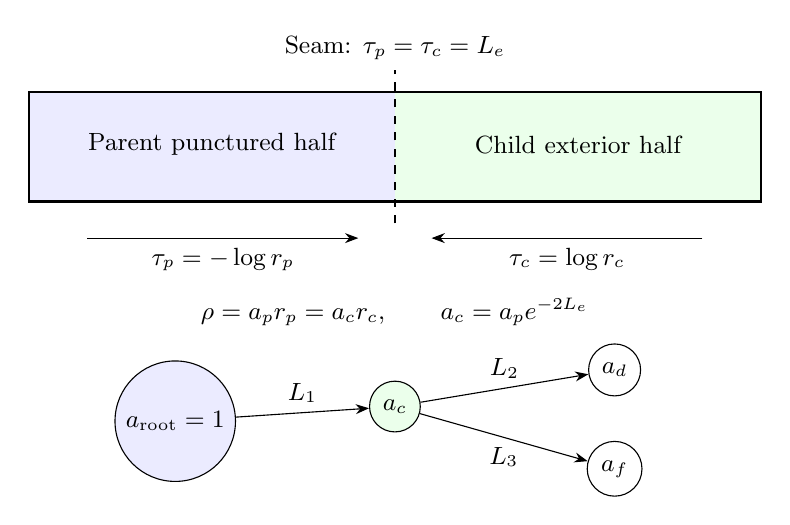
\begin{tikzpicture}[>=Stealth,scale=.93,every node/.style={font=\small}]
 \draw[thick] (0,0)--(10,0);
 \draw[thick] (0,1.5)--(10,1.5);
 \fill[blue!8] (0,0)rectangle(5,1.5);
 \fill[green!8] (5,0)rectangle(10,1.5);
 \draw[thick] (0,0)rectangle(10,1.5);
 \draw[dashed,thick] (5,-.3)--(5,1.8);
 \node at (2.5,.78){Parent punctured half};
 \node at (7.5,.78){Child exterior half};
 \draw[->] (.8,-.5)--(4.5,-.5)node[midway,below]{$\tau_p=-\log r_p$};
 \draw[->] (9.2,-.5)--(5.5,-.5)node[midway,below]{$\tau_c=\log r_c$};
 \node[above] at (5,1.8){Seam: $\tau_p=\tau_c=L_e$};
 \node[below] at (5,-1.18){$\rho=a_pr_p=a_cr_c,\qquad a_c=a_pe^{-2L_e}$};
 \node[circle,draw,fill=blue!8,inner sep=3pt] (r) at (2,-3){$a_{\rm root}=1$};
 \node[circle,draw,fill=green!8,inner sep=3pt] (c) at (5,-2.8){$a_c$};
 \node[circle,draw,inner sep=3pt] (d) at (8,-2.3){$a_d$};
 \node[circle,draw,inner sep=3pt] (f) at (8,-3.65){$a_f$};
 \draw[->] (r)--node[above]{$L_1$}(c);
 \draw[->] (c)--node[above]{$L_2$}(d);
 \draw[->] (c)--node[below]{$L_3$}(f);
\end{tikzpicture}

\caption{A joined parent puncture and child exterior use opposite logarithmic coordinates. Their seam has physical radius $a_p e^{-L_e}=a_c e^{L_e}$ and $a_c/a_p=e^{-2L_e}$. The inset records a finite tree with independently diverging edge lengths; neither relative length ratios nor rates of divergence are fixed. The diagram is schematic.}
\label{fig:tree-scales}
\end{figure}
\FloatBarrier

\section{Selection of paths at several exponential ends}\label{sec:path}

The reduction used to prove Theorem~\ref{thm:tree-inequality} needs a path on
which every original parameter has finite weighted variation.  The parameters
include several independently diverging neck lengths.  Ordinary analytic
curve selection does not directly apply at those ends.  We give the precise
asymptotic class and the selection argument used below.  In particular, the
argument includes the specialization of several lengths; one-variable
quasianalyticity alone would not supply that step.

\subsection{The class of functions and the selection statement}

Put
\[
 Q(A,c)=\{L\in\C:\Re L>A,\ |\Im L|<c(\Re L)^2\}.
\]
An ordinary parameter is a variable in a fixed complex neighborhood of a
finite real point.  A real holomorphic function is one satisfying
\(P(\overline L,\overline z)=\overline{P(L,z)}\).

\begin{definition}\label{path:def-admissible}
An admissible family in \(m\) lengths consists of real holomorphic functions
\(P(L_1,\ldots,L_m,z)\), with the following properties.  These properties
are required for every recursively extracted coefficient as well as for the
initial functions.
\begin{enumerate}[label=\textup{(\roman*)}]
\item The functions are bounded on a product of regions \(Q(A,c)\), locally
uniformly in the ordinary parameters.
\item For each length there is an expansion
\begin{equation}\label{path:eq-expansion}
 P(L,z)\sim\sum_{d\in D_i}e^{-dL_i}
             \sum_{k=0}^{k_d}L_i^k P_{dk}(L_{\widehat i},z).
\end{equation}
Here \(D_i\subset[0,\infty)\) is locally finite, each \(k_d\) is finite,
and \(k_0=0\) if \(0\in D_i\).  For every cutoff \(B\), subtracting the
terms with \(d\le B\) leaves a remainder bounded by
\(C_Be^{-(B+\epsilon_B)\Re L_i}\), for some \(\epsilon_B>0\), on
possibly smaller quadratic regions.  Bounds are uniform on each fixed
smaller ordinary-parameter polydisc.
\item For every subset of expanded lengths, all its coefficient formulas,
at all orders, are holomorphic on one common tail band
\[
 \prod_{j\text{ unexpanded}}
 \{\Re L_j>A',\ |\Im L_j|<c'\},\qquad c'>0,
\]
times one common open ordinary-parameter neighborhood.  These domains may
be shrunk once when a finite number of families are used together.  The
constants and thresholds in asymptotic \emph{estimates} may depend on the
order; the common domains of \emph{analyticity} do not.
\item If a subset of real parts has the form
\(\Re L_i=c_iU+o(U)\), where \(c_i>0\), the corresponding iterated
expansion can be grouped by weights \(\sum_i c_id_i\).  The grouped
weights are locally finite, and each finite cutoff has a remainder of
strictly better exponential order in \(U\).  The assertion holds on the
complex neighborhoods in \textup{(i)} and locally uniformly on the common
ordinary-parameter neighborhood.  It is enough to establish it by
successive single-length expansions.
\end{enumerate}
When \(m=0\), admissible families are ordinary holomorphic germs.
\end{definition}

The distinction in \textup{(iii)} will be used when an expansion has
infinitely many zero coefficients.  It is not an assertion that all
remainder estimates hold beyond a single order-independent threshold.

\begin{theorem}[Path selection]\label{thm:path-selection}
Let \(P_1,\ldots,P_s\) be an admissible finite family, and let a finite
Boolean combination of conditions \(P_j>0\), \(P_j=0\), and \(P_j<0\)
hold along a sequence
\[
 L_i^{(n)}\longrightarrow+\infty,\qquad z^{(n)}\longrightarrow z_0.
\]
There is a real analytic map \(u\mapsto(L(u),z(u))\), defined for all
sufficiently large real \(u\), with the same limits and satisfying those
conditions on its tail.  Each actual coordinate \(L_i(u)\) and
\(z_a(u)\) is eventually monotone or constant.  Given any additional
finite admissible list, its values on the path can also be required to be
eventually monotone or constant.  Finite prescribed limits of functions
can be imposed at the same time.
\end{theorem}

A path germ here means analyticity at every sufficiently large finite
\(u\); analyticity at the limiting endpoint is not asserted.  To impose
\(P\to\ell\), introduce an ordinary variable \(v\to\ell\) and impose
\(P-v=0\).  If there are no length variables, add an unused length.  This
also provides positive infinitesimals for strict sign conditions at an
ordinary limiting point.

\begin{corollary}[The variation consequence]\label{path:variation}
Suppose admissible functions \(F,J\), with \(J\ge0\), satisfy
\[
 |dF|\le C\sqrt J\left(\sum_a|dz_a|
                  +\sum_i e^{-cL_i}|dL_i|\right),\qquad c>0,
\]
on real parameter domains.  There cannot be a sequence with
\(L_i\to\infty\), an interior ordinary-parameter limit, and
\(F\ne0\), \(F^2\ge c_0J\), \(F\to0\), where \(c_0>0\).
\end{corollary}
\begin{proof}
Theorem~\ref{thm:path-selection} realizes all these conditions on one
path with monotone actual coordinates.  Along it,
\[
 |d\log|F||\le\frac C{\sqrt{c_0}}
       \left(\sum_a|dz_a|+\sum_i e^{-cL_i}|dL_i|\right).
\]
Each \(z_a\) has finite total variation because it is monotone with
a finite limit.  Each length tends monotonically to infinity on its
tail, and
\[
 \int_{u_0}^\infty e^{-cL_i(u)}|L_i'(u)|\,du
       =c^{-1}e^{-cL_i(u_0)}<\infty.
\]
Thus \(\log|F|\) has finite total variation and a finite limit, whereas
\(F\to0\) forces \(\log|F|\to-\infty\), a contradiction.
\end{proof}

The remaining subsections prove Theorem~\ref{thm:path-selection}.
The geometric construction resumes in Section~\ref{sec:family} and
uses Definition~\ref{path:def-admissible} and
Corollary~\ref{path:variation} as its analytic interface.

\subsection{Sectors, uniqueness, and clocks}

\begin{definition}\label{path:def-sector}
An admissible angular loss is a positive continuous function \(\omega(r)\), for large
\(r\), such that
\[
 \omega(r)\ge(\log r)^{-2},\qquad
 \sum_{n\ge n_0}\sup_{2^n<r<2^{n+2}}\omega(r)<\infty.
\]
Its sector is the open set
\(S_\omega=\{z:|z|>R,\ |\arg z|<\pi/2-\omega(|z|)\}\).
Every positive loss satisfying the displayed bounds has a continuous
admissible enlargement: at dyadic radii choose a summable majorant of
the neighboring shell suprema and interpolate linearly in \(\log r\).
Thus enlarging a loss to make its sector open only shrinks that sector.
Increasing a loss by a fixed factor or taking a continuous majorant of
the suprema over finitely many neighboring dyadic shells is permitted.  Given finitely many losses we
can dominate all of them by another admissible loss.  We can also arrange
that the domination ratio tends to infinity: if \(a_n\ge0\) is summable,
choose increasing constants \(c_n\to\infty\), sufficiently slowly that
\(\sum c_na_n<\infty\).
\end{definition}

The principle that a bounded holomorphic function is determined by its
exponentially accurate expansion is central to Ilyashenko
quasianalyticity; see~\cite[Fact~1.5]{SpeisseggerQA} in the published
version. We prove the following variant with a summable angular loss,
which is the form preserved by the clock changes below.

\begin{lemma}[Sector uniqueness]\label{path:sector-uniqueness}
Suppose \(f\) is bounded and holomorphic on an admissible sector and, on
the central subsector \(|\arg z|\le\pi/4\), satisfies
\(f(z)=O_B(e^{-B|z|})\) for every \(B>0\).  Then \(f=0\).
\end{lemma}
\begin{proof}
Let \(w_n\) be the supremum of the prescribed loss on a fixed enlargement
of the \(n\)-th dyadic shell.  Choose summable \(a_n\ge0\) with
\(a_n/w_n\to\infty\); enlarge them by a fixed factor if necessary.
On the right half-plane define
\[
 A(z)=\sum_n\frac{a_n}{1+z/2^n},\qquad \Phi(z)=z\exp A(z).
\]
The series is normally convergent there, \(A(z)\to0\) uniformly as
\(|z|\to\infty\), and \(|\Phi(z)|\asymp|z|\).  For \(\Im z>0\),
every summand has nonpositive imaginary part.  If
\(\pi/4\le\arg z\le\pi/2\), the terms with \(2^n\asymp|z|\)
have negative imaginary part of magnitude at least a fixed multiple of
\(a_n\).  Thus the change in argument pushes the outer part of the
half-plane inside the prescribed sector.  Reflection proves the assertion
below the real axis; on the central part it follows from \(A=o(1)\).
Translating the half-plane sufficiently far to the right puts its whole
image in the domain of \(f\).

The bounded pullback \(F=f\circ\Phi\) is superexponentially small on a
fixed central sector, for example \(|\arg z|\le\pi/8\).  In a
half-disc of radius \(r\), the harmonic measure at a fixed positive
interior point of the central part of its semicircular boundary is at
least \(c/r\).  One can see this directly by scaling to the unit
half-disc: the Poisson kernel on a compact subarc away from its endpoints
is comparable to the distance of the rescaled axial point from the
straight boundary, namely a constant times \(1/r\).  Write
\(M\) for a bound for \(|F|\).  On that arc
\(\log|F|\le-Bc_1r+C_B\), and on the rest of the boundary
\(\log|F|\le\log M\).  The subharmonic maximum principle gives
\[
 \log|F(z_*)|\le\log M-c_2B+O_B(r^{-1}).
\]
Zeros cause no difficulty: use the subharmonic function
\(\max\{\log|F|,-N\}\) and then let \(N\to\infty\).
First let \(r\to\infty\), then \(B\to\infty\).  Hence \(F\) vanishes
at every fixed axial point.  The Identity Theorem gives \(F=0\), and
then \(f=0\), since \(\Phi\) is nonconstant and its image is open.
\end{proof}

We now describe the one-variable fields into which the selected paths
will be placed.  Begin with a positive variable \(x_1\to\infty\) and
the field \(B_0\) of convergent meromorphic Puiseux germs in \(1/x_1\).
At stage \(j\), the clock \(x_j\) belongs to \(B_{j-1}\), and for
\(j>1\) it satisfies \(x_{j-1}=o(x_j)\).  The first clock is \(x_1\),
or a positive constant multiple of it.  A germ in \(B_j\) has an
expansion
\begin{equation}\label{path:eq-clock-series}
 f\sim\sum_{\beta\in E}e^{\beta x_j}b_\beta,
 \qquad b_\beta\in B_{j-1},
\end{equation}
where the real set \(E\) is bounded above and finite above each cutoff.
The germ and the continued coefficients are holomorphic on admissible
sectors in the variable \(x_j\).  After a finite cutoff the remainder
has a strictly better exponential rate in \(\Re x_j\), on a possibly
smaller admissible sector.  This includes sector estimates for an empty
expansion.  The same definition is used for holomorphic families on
fixed ordinary-parameter polydiscs, with estimates on smaller polydiscs.
At the Puiseux level a parameter family has a common finite
ramification denominator and pole order, holomorphic coefficient
functions on the ordinary polydisc, and a convergent series locally
uniform there; bounds are taken on smaller polydiscs.

\begin{lemma}[Clock calculus and change of clock]\label{path:clock}
The preceding construction has the following properties, established
simultaneously by induction.
\begin{enumerate}[label=\textup{(\alph*)}]
\item Each \(B_j\) is a field, closed under differentiation in \(x_1\)
and conjugation.  A nonzero scalar has a leading equivalent
\begin{equation}\label{path:eq-leading-monomial}
 Cx_1^p\exp\!\left(\sum_{k=1}^j\beta_kx_k\right),
 \qquad C\ne0,
\end{equation}
uniformly on a suitable admissible sector.  Its real subfield is a Hardy
field: every nonzero real germ has a fixed eventual sign, and its
derivative either vanishes or has a fixed eventual sign.
\item If \(H\in B_j\) is positive and \(x_j=o(H)\), it is a valid
new sector variable.  Finitely many prescribed earlier-clock sectors
can be reached by taking a sufficiently narrow admissible \(H\)-sector.
If \(f\in B_j\) is positive, unbounded, and \(f=O(H)\), then on such
a sector its modulus is comparable to its value at the corresponding
positive real \(H=|H|\); it maps into any finitely prescribed
admissible \(f\)-sectors.  If \(f=o(H)\) on the real ray, then
\(\Re f=o(\Re H)\) throughout the narrowed sector.
\end{enumerate}
\end{lemma}
\begin{proof}
For \(B_0\), inversion and all assertions follow by convergent Puiseux
inversion.  A positive unbounded Puiseux germ is a positive constant
times a positive power of the real variable, with a relative error
tending to zero.  If \(f=O(H)\), the corresponding power is at most the
power for \(H\).  A strictly smaller power leaves a fixed angular
margin.  Equal powers require only an enlarged admissible loss.
Pullback of a loss under comparable positive power growth preserves
dyadic summability.

Assume both assertions at lower levels, and write \(x=x_j\).  Their
change-of-clock assertion permits evaluation of lower germs on
\(x\)-sectors and gives
\(\Re x_k=o(\Re x)\) for \(k<j\).  Consequently every fixed nonzero
lower scalar and its reciprocal have magnitude
\(\exp(o(\Re x))\).  The largest exponent in a nonempty expansion
therefore determines its leading term, separated from the rest by a
positive exponential gap.  Induction gives
Equation~\eqref{path:eq-leading-monomial}.  Sums and products are
calculated termwise: above any cutoff only finitely many pairs of
exponents occur.  To invert, factor the leading term and use a geometric
series in the exponentially small remainder.  A finite desired cutoff
uses only finitely many geometric terms.  A zero expansion is bounded
on the sector supplied by any one of its remainder estimates and
superexponentially small on the central sector.  Lemma~\ref{path:sector-uniqueness}
then makes the germ zero.  Thus the leading-term test is valid also
after cancellation.

Cauchy's formula on successively smaller sectors differentiates each
finite expansion and its remainder.  The radii of the Cauchy discs can
be chosen with logarithmic relative loss, after enlarging the angular
loss on neighboring shells.  Their reciprocal costs, and the
lower-field factor from differentiating the clock, can be absorbed in
an arbitrarily small loss of an exponential remainder rate.  The chain
rule and the induction hypothesis give closure under differentiation
in \(x_1\).  Reflection gives conjugation.  A real leading monomial
has a nonzero real leading constant, hence a fixed sign.  Applying this
to the derivative proves the Hardy-field assertion.  These steps use
only the lower-level change of clock, not the still-to-be-proved
change of clock in \(B_j\).

We prove that change next.  On every strip within a bounded distance
of the real \(x\)-ray, a nonzero lower scalar has ratio \(1+o(1)\) to
its value at a neighboring real point.  Indeed the earlier clocks have
size \(o(x)\), uniformly on fixed proportional discs by the induction
hypothesis, and Cauchy's estimate makes their derivatives \(o(1)\).
The logarithmic derivative of the factor \(x_1^p\) has the same
property.  The leading equivalent and a smaller sector give the
assertion for every nonzero lower scalar.  The assertion applies to a
nonzero lower-field derivative as well; division by \(dx/dx_1\)
expresses differentiation in \(x\) inside the lower field.

Write
\begin{equation}\label{path:eq-H-leading}
 H=e^{bx}h(1+E),\qquad h\in B_{j-1},\quad h>0,
 \quad E=O(e^{-\epsilon\Re x}).
\end{equation}
Since \(H\) is unbounded, \(b\ge0\).  First suppose \(b>0\).
On bounded strips,
\((\log H)'=b+o(1)\).  Analytic inversion along the arcs
\(H=\rho e^{i\theta}\), \(|\theta|\le\pi/2\), gives
\begin{equation}\label{path:eq-clock-inverse}
 x(\rho e^{i\theta})=x(\rho)+i\theta/b+o(1),\qquad
 \partial_\theta x=i/b+o(1),
\end{equation}
uniformly in \(\theta\).  For completeness, solve the inverse equation
first on a fixed small \(\theta\)-interval by the Analytic Inverse
Theorem, using the uniform lower bound \(|(\log H)'|\ge b/2\).
Continue over finitely many such intervals.  Integrating the inverse
derivative gives Equation~\eqref{path:eq-clock-inverse}, keeps the
solution in a bounded strip, and guarantees uniqueness on overlaps.
The resulting branches agree with the real inverse and hence agree
where their sector domains overlap.

If \(f=e^{ax}g(1+O(e^{-\epsilon'\Re x}))\), where \(g>0\) is lower
level, then unboundedness and \(f=O(H)\) give \(0\le a\le b\).
When \(a<b\), its argument tends uniformly to \(a\theta/b\), so
there is a fixed angular margin.  Its real size relative to \(H\)
decays exponentially in \(x\), which proves real-part separation even
after division by a logarithmic angular margin.  When \(a=b\), put
\(J=g/h\).  This is a positive bounded lower scalar, and
\[
 f/H=J(1+O(e^{-\epsilon_1\Re x})).
\]
The strip estimate implies, uniformly for \(|\theta|\le\pi/2\),
\[
 \frac{\Re f}{|H|}
   =O(J(x(\rho))\cos\theta)
     +O(|J'_x(x(\rho))|+e^{-\epsilon_2x(\rho)}).
\]
If \(J\to0\), its derivative is eventually negative unless it is
zero.  More precisely, put \(q=J'_x/J\), \(t=x(\rho)\), and
\(D=(\log H)'\).  Equation~\eqref{path:eq-clock-inverse} and the
strip estimate give
\[
 \frac{d}{d\theta}\arg J(x(\rho e^{i\theta}))
   =\Re\frac{q(x(\rho e^{i\theta}))}{D(x(\rho e^{i\theta}))}
   =\frac{q(t)}b(1+o(1)).
\]
Thus its phase changes toward the real axis for positive \(\theta\);
reflection handles negative \(\theta\).
If \(J\) has a positive limit, either direction of its vanishing
phase error is allowed.

The strip estimate also gives
\(J(x(\rho e^{i\theta}))=J(t)+O(|J'_x(t)|)\), and hence
\[
 \frac{|\Re f|}{\Re H}
 \le C J(t)+C\frac{|J'_x(t)|+e^{-\epsilon_2t}}{\omega_H(\rho)}.
\]
Choose the angular loss for \(H\) to dominate
\(|J'_x|+e^{-\epsilon_2x}\) by a factor tending to infinity.  This is
an admissible choice.  In fact \(J\) is eventually monotone with a
finite limit, so \(\int|J'_x|\,dx<\infty\).  Its suprema on bounded
\(x\)-intervals are comparable to its integrals there, by the strip
estimate for the derivative; a zero derivative needs no estimate.
Since \(\log H=bx+o(x)\) and its derivative tends to \(b\), these
intervals correspond to dyadic \(H\)-shells.  The preceding displayed
estimate now gives \(\Re f=o(\Re H)\) when \(J\to0\).  Prescribed
losses for the \(f\)-sector can also be pulled back: here
\(d\log f/d\log H\to1\), so a dyadic shell in either variable meets
only a bounded number of shells of comparable logarithmic width in
the other.  Their pulled-back suprema are summable.  Enlarging the
\(H\)-loss once more gives the sector mapping and modulus assertions.

It remains to consider \(b=0\).  Use \(h\) first as variable at the
previous level.  It is larger than \(x\), and \(\log h=o(x)\), because
the logarithm of a lower scalar is controlled by earlier clocks.
The lower change-of-clock assertion applies both to \(x\) and to the
leading lower factor of \(f\); \(f\) also has top exponent zero.
In the \(h\)-variable, the map from \(h\) to \(H\) in
Equation~\eqref{path:eq-H-leading} is a relative perturbation
\(O(e^{-\epsilon\Re x})\).  Take a wider and a narrower admissible
sector with margins at least a fixed multiple of
\((\log|h|)^{-2}\).  On the wider sector
\[
 \Re x\gtrsim |x|(\log|x|)^{-2},\qquad
 |x|\asymp x(|h|).
\]
Here are quantitative inverse estimates.  At a target point \(H_0\)
put \(r=|H_0|\), \(w=\log r\), \(X_0=x(r)\), and
\(\rho=cw^{-2}\).  Enlarge the losses on neighboring shells so that
\(D(H_0,4\rho r)\) lies in the wider sector.  The positive harmonic
function \(\Re x\) satisfies Harnack's inequality there, so on
\(D(H_0,2\rho r)\) the perturbation is bounded by
\[
 \eta=C\exp\{-c_1\epsilon X_0/(\log X_0)^2\}.
\]
Since \(w=o(X_0)\), one has \(\eta w^N\to0\) for each fixed
\(N\).  Rouch\'e's Theorem on a disc of radius \(\rho r\),
followed by Cauchy's estimate, gives a unique nearby inverse \(u\)
with
\[
 |u-H_0|=O(\eta r),\qquad
 \frac{dH}{dh}(u)=1+O(\eta/\rho).
\]
Uniqueness glues these inverse branches on overlaps.  For any positive
unbounded lower factor \(F=O(h)\), its sectorial logarithm is
\(O(w)\).  Cauchy's estimate therefore gives
\[
 |\log F(u)-\log F(H_0)|=O(\eta w^3)=o(w^{-2}).
\]
This proves modulus comparability and preserves every enlarged angular
margin.  If \(F=o(h)\), induction gives \(\Re F(u)=o(\Re u)\),
whereas \(\Re u/\Re H_0=1+O(\eta w^2)\).  The extra relative
exponential perturbation in \(f\) contributes at most \(O(\eta w^2)\)
after division by \(\Re H_0\), using a smaller common exponential
rate for the finitely many functions.  Thus real-part separation is
unchanged.  This completes the simultaneous induction.
\end{proof}

Only finitely many sector requirements are imposed at a time in
Lemma~\ref{path:clock}.  Different truncation orders may use different
losses and different initial radii.

\begin{lemma}[Sectorial limits of holomorphic families]
\label{path:family-limits}
Let \(F\) be a holomorphic family in a finite clock hierarchy,
on an ordinary polydisc \(D\).  Suppose that on the positive path
ray it converges to a finite holomorphic family \(F_\infty\),
locally uniformly on \(D\).  Then on every fixed smaller polydisc
\(D'\Subset D\), it converges uniformly to the same family on
some admissible sector of its last clock.  The conclusion remains
valid after passing to a faster admissible clock by
Lemma~\ref{path:clock}.  Finitely many such requirements can be
imposed on one sector.  In particular, a normalized limit which
is nonzero on a fixed compact contour stays uniformly nonzero
there, and finitely many composition arguments with limiting
images in prescribed open domains stay in those domains.
\end{lemma}
\begin{proof}
First note a uniform growth consequence of the parameter expansion
calculus.  A lower-level family, together with any fixed finite list
of its ordinary derivatives, is \(\exp(o(\Re x_j))\) on a suitable
sector of a faster clock \(x_j\), uniformly on a smaller ordinary
polydisc.  At the Puiseux level convergence gives a polynomial bound
in the first clock.  At a higher level take a finite cutoff below
the largest exponent.  There are only finitely many retained lower
coefficient families; their inductive bounds and the prescribed
remainder bound control the family by an exponential in its last
clock.  After passing to \(x_j\), Lemma~\ref{path:clock} makes the
real parts of all these earlier clocks \(o(\Re x_j)\); its modulus
comparability treats the polynomial factors.  Cauchy's formula on
one fixed smaller ordinary polydisc gives the same assertion for
any specified finite derivative list.  No nonzero normalization of
these families is required for this upper bound.

We now prove the finite-limit assertion by induction on the hierarchy.
At the Puiseux level, real-ray boundedness eliminates negative powers
of the small ramified variable.  The convergent series with holomorphic
coefficients then converges to its constant term also for complex
small argument, locally uniformly in the ordinary parameters.

At level \(j\), write the expansion as
\(\sum_\beta e^{\beta x_j}B_\beta\).  If a positive exponent has a
nonzero coefficient family, choose the largest such exponent and an
ordinary Taylor coefficient of \(B_\beta\) which is a nonzero scalar
germ.  Cauchy's formula makes the corresponding Taylor coefficient
of \(F\) bounded on the positive ray.  Its scalar expansion, however,
has a positive leading top exponent and a nonzero lower scalar
coefficient.  That coefficient and its reciprocal are subexponential
in \(x_j\) by Lemma~\ref{path:clock}, contradicting boundedness.
Zero coefficient families can be discarded; finiteness above each
cutoff ensures that the largest nonzero positive exponent exists if
there is one.  Thus every positive top coefficient vanishes.

Take the cutoff at zero and put \(B_0=0\) when that weight is absent.
The strict remainder gain gives
\[
 F=B_0+O(e^{-\epsilon\Re x_j})
\]
uniformly on a smaller ordinary polydisc and a suitable sector.  If
a truncation convention retains finitely many negative terms as well,
the preliminary uniform subexponential bound absorbs those terms
into this estimate with a smaller positive \(\epsilon\).
Consequently \(B_0\) has the same finite locally uniform limit on
the positive ray as \(F\).  By induction it has that limit on a
sector of the preceding clock.  Map the \(x_j\)-sector into this
sector by Lemma~\ref{path:clock}.  Modulus comparability ensures that
the preceding clock tends to infinity uniformly there.  This proves
convergence of \(B_0\), however slow its real-ray rate may be.
The displayed remainder tends uniformly to zero because
\(\Re x_j\gtrsim|x_j|/(\log|x_j|)^2\to\infty\).  The induction
is complete.

A further faster clock maps into the sector just obtained and sends
its tail to uniformly large moduli there, again by
Lemma~\ref{path:clock}.  Thus the limit persists.  A finite collection
of requirements uses a common admissible majorant of the finitely
many losses and a common sufficiently large radius.  Finally, the
modulus of a limiting unit has a positive minimum on a compact
contour.  Apply uniform convergence on a finite covering by smaller
ordinary polydiscs to make the error less than half this minimum.
For a composition argument choose a compact neighborhood of its
limiting image inside the prescribed domain and apply the same
uniform convergence.  These are finitely many requirements, as
claimed.
\end{proof}

\subsection{Regular systems and finite analytic operations}

We now collect the properties that must survive when another length is
introduced. Every nonzero analytic family must have a scalar
normalization; finite analytic operations must preserve controlled
domains; and the resulting expressions must still be realizable on
paths of the clock class. The definition below makes these requirements
an induction invariant. Preparation and root extraction will then be
finite operations within that invariant.

Fix a nonprincipal ultrafilter \(\mathcal U\) on the indices of the
given sequence.  Such a filter exists by the maximal principle applied
to the cofinite filter.  For every subset of indices, exactly one of
that subset and its complement lies in \(\mathcal U\).  Compactness
therefore gives limits in compact spaces, including the extended real
line.  All comparisons made at the distinguished sequence in the
construction below are in this sense.  Only a finite number of these
comparisons is used to construct any particular path.

\begin{definition}\label{path:def-regular}
A domain base is a directed family of connected real open domains in
auxiliary independent variables, each containing the distinguished
sequence for a set of indices in \(\mathcal U\).  A germ on the base is
an analytic function on one such domain, with its local complexification;
two functions are identified if they agree on a smaller domain.  Extra
ordinary variables range over complex polydiscs about specified standard
values.

A regular system \(\mathcal A\), with scalar field \(K\), has the
following properties.
\begin{enumerate}[label=\textup{(R\arabic*)}]
\item Every nonzero family \(F(q,\zeta)\) admits a nonzero scalar
\(k\in K\) such that \(F/k\) has a finite, nonzero holomorphic limit
as a germ in \(\zeta\), locally uniformly on a polydisc, along the
domain base.  The scalar reciprocal \(1/k\) is in the system.  For
real families \(k\) can be chosen real.  Every scalar comparison or
finite scalar limit made at the distinguished sequence holds along the
base after the appropriate restrictions.
\item For every positive scalar size \(a\) and integer \(n>0\), there
is a positive scalar \(\rho\) with \(\rho^n/a\) tending to a finite
positive constant.  Scalars and reciprocals have magnitude at most
\(\exp(C\max_i L_i^*)\), where \(L_i^*\) are the current centers.
For an empty tuple the bound is constant.
\item The system is closed under finite sums and products, reflection,
ordinary holomorphic composition at finite limiting arguments, inversion
after a nonvanishing normalized limit has been specified, and Cauchy
integration on fixed compact contours.  Integrals over fixed compact
segments are allowed by a finite cover of their holomorphic parameter
neighborhoods.  Domain restrictions for these operations are part of
the finite data of the expression.
\item Given a domain and finitely many normalization, comparison, and
limit requirements, there are families of real analytic paths eventually
in that domain preserving them.  The expressions used belong on each
path to a clock hierarchy of Lemma~\ref{path:clock}, with parameter
versions for any finite specified uses.  The path families have real
constant parameters in open sets and are analytic in those constants
where defined.  At every sufficiently large fixed path time, their
evaluation into the independent-variable domain is locally submersive.
The starting time may depend on the constants.
\end{enumerate}
Limits of families in \textup{(R1)} mean uniform limits on each fixed
smaller polydisc.  A nonzero holomorphic limit need not be nonzero at
its central point.  An inverse requires nonvanishing on the particular
polydisc or contour where that inverse is used.
\end{definition}

The expression ``finite analytic operation'' always includes its inputs
and the domain data needed for them.  This prevents an implicit request
to preserve infinitely many normalizing comparisons on a path.  Two
elementary consequences will be useful.

\begin{lemma}[Preparation on fixed contours]\label{path:prepared-contours}
Let \(F(q,\zeta,y)\) belong to a regular system.  Suppose that after
scalar normalization its limiting germ is regular of degree \(d\) in
the \(y\)-direction at \((\zeta,y)=(0,0)\).  Then its Weierstrass
polynomial, its unit, and division of any other family by that polynomial
are obtained by the operations in \textup{(R3)} on fixed contours and
fixed smaller parameter polydiscs.  Arbitrarily high Taylor coefficients
of these operations use the same denominator zero sets and the same
contours.
\end{lemma}
\begin{proof}
Choose a circle \(|y|=r\) on which the limiting germ is nonzero and
inside which it has precisely \(d\) zeros at \(\zeta=0\), counted
with multiplicity.  After shrinking the \(\zeta\)-polydisc and the
domain in the base, normalized \(F\) is uniformly nonzero on that
circle.  The power sums of its enclosed roots are
\[
 s_\ell(q,\zeta)=\frac1{2\pi i}\int_{|y|=r}
        y^\ell\frac{\partial_yF(q,\zeta,y)}{F(q,\zeta,y)}\,dy,
 \qquad 1\le\ell\le d.
\]
Newton's identities give the monic polynomial \(W\) from these power
sums, by finite polynomial operations.  The quotient \(F/W\) is a
holomorphic unit on a smaller disc by cancellation of the enclosed
zeros; its values there can also be expressed by a fixed-circle Cauchy
formula.  A useful explicit division formula for a holomorphic family
\(G\) is
\[
 G(y)=W(y)\frac1{2\pi i}\int_{|w|=r}
       \frac{G(w)}{W(w)(w-y)}\,dw
   +\frac1{2\pi i}\int_{|w|=r}
       \frac{G(w)}{W(w)}\frac{W(w)-W(y)}{w-y}\,dw.
\]
The second term is a polynomial in \(y\) of degree less than \(d\).
These formulas prove the asserted closure.  Differentiating or expanding
them introduces powers of the existing nonzero contour denominators,
not new denominators with new zero sets.  All Taylor orders are
holomorphic on the same smaller polydisc; their Cauchy constants may
depend on the order.
\end{proof}

\begin{lemma}[Roots in a regular scalar system]\label{path:roots}
Suppose \textup{(R1)--(R3)} hold, including divisibility of positive
sizes.  Then the complex scalar field is algebraically closed and its
real part is real closed.
\end{lemma}
\begin{proof}
We factor monic polynomials by induction on degree.  Translate the
variable to remove the coefficient of degree \(d-1\).  If all the
remaining coefficients vanish, the polynomial is a pure power and the
claim follows.  Otherwise write it as
\[
 y^d+\sum_{j=2}^d a_jy^{d-j}.
\]
Choose, from finitely many positive root-size representatives of the
nonzero \(a_j\), one of largest size, denoted \(\rho\).  Replacing
\(y\) by \(\rho v\) makes all coefficients bounded and makes at
least one non-leading coefficient have a nonzero limit.  The limiting
depressed polynomial has at least two distinct roots: a polynomial
with a single root is \((v-c)^d\), and its vanishing degree-\(d-1\)
coefficient forces \(c=0\).

Choose disjoint small fixed circles around the distinct limiting roots.
The contour power sums used in Lemma~\ref{path:prepared-contours}
give monic factors for the corresponding clusters.  Their coefficients
are in the system, and all their degrees are strictly smaller than
\(d\).  Induction factors each cluster completely.  Undo the scaling
and translation.  For a real polynomial, conjugation pairs the
nonreal factors and fixes every real-valued root.  The real scalar
field is ordered by eventual sign.  Every positive element has a real
square root, and every odd-degree real polynomial has a real root:
at the real points of a sufficiently small base domain these assertions
hold for the factorizations just constructed, and the finite sign and
conjugacy alternatives can be fixed on the domain base.  These two
properties characterize a real closed ordered field.
\end{proof}

\begin{lemma}[Detection of analytic identities]\label{path:detection}
Path families with the submersivity property in \textup{(R4)} detect
analytic germs.  Namely, if an analytic function vanishes on the tail
of every path in such a family, then it vanishes as a domain germ.
The same holds for a holomorphic family in extra ordinary variables.
\end{lemma}
\begin{proof}
Let \(V\) be an open parameter set for one family and use integer path
times \(N\).  At a fixed \(N\), evaluation is analytic on an open
subset \(V_N\subset V\).  On the subset where its differential is
surjective, the composition with a nonzero domain germ is a nonzero
real analytic function on every connected parameter neighborhood:
otherwise submersivity would give an open set of zeros in the domain.
The zero set of a nonzero real analytic function has Lebesgue measure
zero.  This last fact follows by induction on the number of variables:
in one variable zeros are discrete; in higher dimension separate the
points where a nonzero Taylor coefficient in the last variable is
nonzero and use the one-dimensional result and Fubini, with induction
on the exceptional coefficient-zero set.

Every parameter lies, for all sufficiently large integers, in a
submersive evaluation domain and in the zero set of the composition.
If the original germ were nonzero, countably many local parameter
charts for these integer evaluations would thus cover \(V\) by sets
of measure zero, a contradiction.  An open set of domain zeros makes
the germ zero by connectedness and the Analytic Identity Theorem.
For a family in extra variables, apply this argument to each of its
Taylor coefficients, or fix the extra variables in a countable dense
set and then use continuity.
\end{proof}

\subsection{Adjoining a reciprocal fastest length}

The next Lemma is the analytic specialization step.  It is stated with
its quantitative separation hypothesis, since that hypothesis rules out
uncontrolled cancellation against the lower field.

\begin{lemma}[One independent reciprocal]\label{path:adjoin-p}
Let \(\mathcal A\) be a regular system for a nonempty lower tuple
\(L'=(L'_1,\ldots,L'_r)\), with real scalar field \(K_{\R}\).
Assume that each \(L'_i\) is a positive unbounded element of
\(K_{\R}\), and put \(M'=1+\sum_{i=1}^rL'_i\).  Assume in addition
that, for every finite use of its path property, the lower paths can
be chosen with last clock \(x_{\rm prev}=O(M')\).  This is an
additional property of the length systems constructed below; it is
not part of the abstract conditions \textup{(R1)--(R4)}.
Let a new independent positive variable \(p\) have the distinguished limits
\[
 p\longrightarrow0,\qquad p\max L'\longrightarrow0,
 \qquad |p-c|\gtrsim p^2\quad(c\in K_{\R}).
\]
The constant in the last comparison may depend on \(c\).  Use domain
fibers in \(p\) which are open intervals cut out by finitely many
strict comparisons with lower scalars.  There is a regular system
\(\mathcal A[p]\) containing the lower system and \(p,p^{-1}\),
closed under the finite analytic operations, with the following size
bound for each nonzero scalar and its reciprocal:
\begin{equation}\label{path:eq-p-size}
 |a|+|a|^{-1}\le e^{C(1+\max L')}p^{-C}.
\end{equation}
Its finite path requirements can be realized by substituting for \(p\)
an expression in lower scalars, with an additional real constant varying
in an open interval, and preserving \(pM'\to0\).  On the resulting
lower paths one therefore has \(px_{\rm prev}\to0\).

For the empty lower tuple the same conclusion holds with ordinary
holomorphic germs and the choice \(p=\theta/x_1\), \(\theta>0\).
\end{lemma}
\begin{proof}
We give the chart construction, the normalization argument, and the
path argument separately.  Real closedness of the lower field is
available from Lemma~\ref{path:roots}.

\emph{Charts and their common refinements.}
For a real center \(c\in K_{\R}\), let \(s=|p-c|\); fix its sign on
the domain base.  If \(s\) is comparable to a positive lower scalar,
use a disc coordinate
\[
 u=(p-c)/R
\]
with finite limiting value, where \(R>0\) is in \(K_{\R}\).  If no
positive lower scalar has size comparable to \(s\), call the size
unmatched and use a ramified annular chart
\begin{equation}\label{path:eq-annulus}
 u=(s/R)^{1/n},\qquad v=(r/s)^{1/n},\qquad u,v\longrightarrow0,
\end{equation}
where \(R,r\) are lower positive scalars, \(r=0\) is allowed, and the
positive real branches are used.  In the latter chart permit scalar
prefactors \(ks^q\), with \(k\in K\), \(q\in\mathbb Q\).  Functions
are lower analytic families in these bounded coordinates, at their
specified standard values, times such prefactors.  Disc charts require
only lower scalar prefactors.

Here is the finite refinement rule.  Include zero and every center in
the finite data, and choose a center whose distance from \(p\) is
smallest in order.  If its distance is matched, a disc at that scale
expresses all other required coordinates by bounded analytic
substitutions, after normalizing their nonzero distances.  In the
unmatched case each nonzero difference of two centers is either
\(o(s)\) or much larger than \(s\): it cannot be comparable to \(s\),
since that would match \(s\) with a lower scalar.  Write
\[
 p-c'=(p-c)+(c-c')
\]
as the larger term times one plus the smaller ratio.  Choose annular
bounds \(r\ll s\ll R\) recording every one of these finitely many
ratios.  Rational powers are analytic in the factor tending to one,
and a common root denominator handles all ramification.  A required
bounded ratio of prefactors is treated in exactly this way: a ratio
\(ks^q\) has, for \(q\ne0\), a threshold at a lower root-size
representative of \(|k|^{-1/q}\).  Add these finitely many thresholds
to the bounds \(r,R\).  This proves the common-refinement rule,
including bounded analytic representation of every needed ratio.

\emph{Normalization in an annulus.}
On the relation \(uv=\lambda=(r/R)^{1/n}\), decompose a bounded
lower analytic family \(H(u,v,\zeta)\) as
\[
 H_+(u,\zeta)+H_-(v,\zeta),
\]
where the second series has only positive powers of \(v\).  This is
an actual convergent decomposition on a smaller bidisc.  For example,
substitute \((w,\lambda/w)\) on a fixed circle in the original
\(u\)-disc and take its nonnegative Laurent part by Cauchy projection;
the negative part is the positive series in \(v\).  Both belong to
the lower system, since \(\lambda\) is a bounded lower scalar and
the circle is fixed.  If \(r=0\), set \(v=0\) and use just the first
series.

Normalize a nonzero one of these families in the lower system, with
its series variable still ordinary.  Let \(N\) be the first degree
whose coefficient has nonzero standard holomorphic limit in
\(\zeta\).  The terms of degrees less than \(N\) have finitely many
lower scalar normalizers.  The tail beginning at degree \(N\),
factored by that power, is bounded with nonzero standard limit at the
origin.  Thus only finitely many candidate sizes occur.  Distinct
powers of \(s\) cannot have comparable sizes after lower scalar
multiplication: such a comparison, together with divisibility of lower
sizes, would match \(s\).  Choose the largest candidate size over
both Laurent parts.  It is unique up to terms with the identical
power, which are combined before this comparison.  All smaller
candidate ratios have zero limit, and the factored tails remain
bounded by the refinement rule.  Division by the largest size
therefore gives a bounded analytic representation with nonzero
holomorphic standard limit.  If both projected series vanish, the
original family vanishes.

\emph{Normalization in a disc.}
Translate the disc coordinate to have limit zero and normalize the
family \(H(u,\zeta)\) in the lower system before substituting \(p\).
If it is nonzero, choose a Taylor coefficient \(b(u)\) in \(\zeta\)
whose standard limit is a nonzero germ in \(u\).  Preparation and
division in \(u\), by Lemma~\ref{path:prepared-contours}, give
\begin{equation}\label{path:eq-disc-division}
 H(u,\zeta)=b(u)G(u,\zeta)+S(u,\zeta),
\end{equation}
where \(G\) is bounded and \(S\) is a polynomial in \(u\).  Also
\(b\) is a unit times a monic polynomial in \(u\).

The finite-dimensional \(K\)-span of the coefficient germs in
\(\zeta\) of \(S\) has a basis \(\psi_1,\ldots,\psi_h\) whose
standard limits are linearly independent over \(\C\), with each
\(\psi_j\) bounded.  To construct it, normalize a nonzero element,
choose one of its Taylor coefficients with nonzero limit, and normalize
that coefficient to be one.  Pass to the kernel of the corresponding
coefficient functional in the original span and repeat.  The dimension
drops by one at each step.  The resulting triangular Taylor-coefficient
matrix has nonzero limiting diagonal, proving the assertion.  Hence
\[
 S(u,\zeta)=\sum_{j=1}^h A_j(u)\psi_j(\zeta),
\]
where the \(A_j\) are polynomials over \(K\); its size after
specialization is the largest of their nonzero sizes.

Factor these finitely many polynomials, together with the polynomial
for \(b\), over \(K\).  Include the real parts of their roots, expressed
in the \(p\)-coordinate, among the centers of the refinement.  The
imaginary parts are lower scalars; their sizes are additional comparison
thresholds.  Every factor then has a bounded normalized analytic
representation, using either a disc or an annulus.  The largest size
among \(b,A_1,\ldots,A_h\) normalizes \(H\).  If an \(A_j\)-size
strictly dominates that of \(b\), independence of the standard
\(\psi_j\) prevents cancellation.  Otherwise \(b\) itself is a
Taylor coefficient of \(H\), so a normalized limit of \(H\) cannot
vanish identically.  The boundedness of the representation and Cauchy's
formula make this coefficient argument valid for holomorphic limits.

\emph{Bounds and analytic closure.}
All resulting sizes are products of lower scalar sizes and rational
powers of distances and scales.  Every nonzero distance from \(p\)
to a real lower center is at least a fixed multiple of \(p^2\).
Upper bounds for centers and scales, and bounds for their reciprocals,
are lower exponential bounds.  The preceding finite factorizations
therefore give Equation~\eqref{path:eq-p-size}.  Positive root-size
representatives follow from ramification and the lower representatives.
For a bounded scalar the chart formula gives its finite standard
limit; prefactor ratios are controlled by the recorded comparisons.
Nonzero real scalars have a fixed sign.  A complex normalizer for a real
family can be replaced by a real or imaginary part of comparable size,
and then by a positive representative if desired.

After common refinement, sums, products, ordinary composition, and
normalized unit inversion are the corresponding lower analytic
operations on bounded families.  Contour integrals are treated by
finitely many chart neighborhoods covering the contour.  The same
argument works for a compact segment.  This proves
\textup{(R1)--(R3)} for the extension.  Comparisons such as
\(|p-c|\gtrsim p^2\) can be expressed by interval endpoints in the
real lower field: factor the relevant real polynomial inequalities
using Lemma~\ref{path:roots}, order their roots, and choose the interval
containing the distinguished points.

\emph{Finite specialization and path families.}
Refine using all chart centers, all endpoints of the required interval,
and zero.  In a matched chart, with positive scale \(d\) and limiting
coordinate \(a\), choose
\begin{equation}\label{path:eq-matched-choice}
 p=c+ad+\theta d\eta,
\end{equation}
where \(\eta>0\) is a lower infinitesimal and \(\theta\) varies in a
small open interval of constants.  Its sign can be fixed to meet the
fiber constraints.  Every included endpoint has nonzero normalized
distance at its own recorded scale.  Choose \(\eta\) smaller than
the finitely many required relative margins.  Then all comparisons
persist and every required coordinate has its exact limiting standard
part.  If an endpoint were nearer than the chosen center-scale data,
it would already have been selected by the closest-center refinement;
thus this choice omits no cancellation relevant to the finite data.

In an unmatched chart choose a lower scale strictly between all
required lower and upper bounds, for instance their geometric mean
after taking the largest lower and smallest upper bound.  If the lower
bound is zero, multiply the upper bound by a positive lower
infinitesimal.  Set \(s\) equal to this scale times \(\theta\) in a
bounded positive open interval, and set \(p=c\pm s\) with its recorded
sign.  Thresholds required by bounded prefactors were already included,
so these substitutions preserve all finite normalization requirements.
They use only lower scalar and ordinary analytic operations.

Include among the finite requirements \(p\to0\) and \(pM'\to0\).
The latter uses only the already defined positive lower scalar
\(M'\): it is the requirement \(p/(1/M')\to0\), handled by the
same disc or annular refinement.  The lower system contains positive
infinitesimals, for example \(1/M'\).  Apply the lower path property,
with its assumed clock bound, to these and all other expressions and
comparisons used in the chosen substitutions.  Then
\(px_{\rm prev}=O(pM')\to0\); no comparison involving a clock
chosen only later is imposed on the domain base.
Formula~\eqref{path:eq-matched-choice}, or
its unmatched counterpart, has nonzero derivative in the new constant
\(\theta\).  Together with submersivity of the lower evaluation,
the triangular differential gives submersivity into the extended
domain.  Interval fibers over connected lower domains are connected
after ordering their endpoints; they remain the domain base under
these restrictions.  This proves \textup{(R4)}.  In the empty case,
  \(p=\theta/x_1\) gives the stated meromorphic Puiseux families directly.
\end{proof}

\subsection{Construction for several lengths}

We now construct the regular system of
Definition~\ref{path:def-regular} for the original tuple of length
variables. The induction separates lengths of comparable size from
strictly slower differences, applies the reciprocal-length construction
when necessary, and preserves the common coefficient domains. Its
output will leave only the ordinary-variable sign conditions to solve
in the final subsection.

For example, the admissible equation
\[
 e^{-L_1}-L_2e^{-L_2}=0
\]
has the path \(L_2=e^u\), \(L_1=e^u-u\).
The lengths have ratio tending to one, but their difference is the
unbounded slower quantity \(-u=-\log L_2\). Thus grouping lengths by
their limiting ratios must retain the magnitudes of unbounded slower
differences as new centers.

\begin{proposition}[Centers and regular systems]\label{path:centers}
For a distinguished sequence of \(m\) lengths tending to infinity,
there are centers \(L_1^*,\ldots,L_m^*\), differing from the sequence
values by bounded additive amounts, and a regular system on a domain
base with the following additional properties.
\begin{enumerate}[label=\textup{(\alph*)}]
\item The system contains the centers, \(e^{bL_i^*}\) for every real
\(b\), and every admissible family evaluated at these centers.
\item Every finite expression built with the allowed analytic
operations has coefficient formulas on a common connected domain of
the base and a common ordinary-parameter neighborhood.  The same
formulas remain valid to all orders on paths preserving its finite
preparation data.  Remainder sectors and thresholds may depend on
order.
\item On the path families, the grouped centers have the form
\(c_iX+D_i^*\), \(c_i>0\), where the positive magnitudes of the
unbounded \(D_i^*\) are slower centers.  All required quadratic
holomorphy domains are reached after narrowing the clock sectors.
\item For a nonempty tuple, its path families can be chosen so that
the last clock is the selected fastest center \(X\).  Every center
is \(O(X)\), and one of the centers equals \(X\).  In particular
the last clock is comparable to \(\max_iL_i^*\), independently
of which finite expression requirements are imposed.
\end{enumerate}
\end{proposition}
\begin{proof}
We induct on \(m\), establishing all regularity and path assertions
together, including the last-clock invariant in \textup{(d)}.
The empty tuple has ordinary holomorphic germs, constant
scalars, and a point as its independent-variable domain.  Its
normalization and contour assertions are immediate; the path assertion
has zero-dimensional target and is vacuous.

\emph{Splitting the fastest block.}
Choose a fastest length \(X\), so that every ratio \(L_i/X\) has
a finite ultrafilter limit.  This is possible by taking a maximal
one among the finitely many lengths.  For the indices with positive
limit write
\[
 L_i=c_iX+D_i,\qquad c_i>0,\quad D_i=o(X).
\]
Ignore bounded \(D_i\) for now, replacing them by zero in the centers.
For each unbounded difference take its absolute value and record its
eventual sign.  These magnitudes and the lengths with ratio zero to
\(X\) form a lower tuple of at most \(m-1\) entries.  Indeed a
fastest block of size \(k\) contributes at most \(k-1\) differences,
and the other block has \(m-k\) lengths.  Apply the induction
hypothesis to that tuple and denote the resulting positive centers by
\(L'\).  Reinsert the recorded signs in the differences \(D_i^*\).

If some real lower scalar approximates the original \(X\) to bounded
absolute error, replace \(X\) by it.  Its positivity, its divergence,
and \(\max L'=o(X)\) are finite lower-system requirements.  Otherwise
adjoin \(p=1/X\) as an independent variable.  For every real lower
scalar \(c\),
\begin{equation}\label{path:eq-separation}
 |p-c|\gtrsim p^2.
\end{equation}
In fact failure, or even a bounded ultrafilter value of
\(|p-c|/p^2\), would give \(c/p\to1\) and
\[
 X-1/c=\frac{c-p}{pc}=O(1),
\]
contrary to the case distinction.  Thus Lemma~\ref{path:adjoin-p}
applies.  In both cases call the resulting coefficient system
\(\mathcal A'\).  Every nonzero scalar of \(\mathcal A'\), and its
reciprocal, is \(e^{o(X)}\), by
Equation~\eqref{path:eq-p-size}, \(\max L'=o(X)\), and
\(\log X=o(X)\).  The final centers in the fastest block are
\(c_iX+D_i^*\), including \(X\) itself.  All errors relative to the
distinguished original tuple are bounded.

\emph{Initial grouped expansions and their domains.}
Adjoin \(e^{\alpha X}\), \(\alpha\in\R\), and the initial
admissible functions evaluated at the centers.  Their fastest-block
expansions have the form
\begin{equation}\label{path:eq-grouped}
 \sum_d e^{-dX}B_d,\qquad B_d\in\mathcal A',
\end{equation}
with locally finite weights and strict exponential remainder gains.
To obtain the coefficient, expand a term with fastest-block indices
\(d_i\) as
\[
 \prod_i e^{-d_i(c_iX+D_i^*)}(c_iX+D_i^*)^{k_i}.
\]
Its top exponential is \(e^{-(\sum_i c_id_i)X}\).  Its remaining
factors are polynomials in \(X,D_i^*\), exponentials of the signed
lower centers, and recursively extracted initial coefficients in the
slower lengths.  All are in \(\mathcal A'\).  Definition~\ref{path:def-admissible}
supplies both the grouped remainder and the common analytic domains
of every coefficient formula.

The inductive lower construction supplies
\(x_{\rm prev}=O(1+\sum_iL'_i)\), and contains the positive lower
centers as real scalars.  Thus it meets the additional hypotheses of
Lemma~\ref{path:adjoin-p}.  In the independent case that specialization
preserves \(p(1+\sum_iL'_i)\to0\); hence
\(x_{\rm prev}=o(X)\), where \(X=1/p\).  In the dependent case
\(X\) is a lower scalar, and the already required comparison
\((1+\sum_iL'_i)/X\to0\) can be imposed using the lower path
property; it again gives \(x_{\rm prev}=o(X)\).  Thus in either
case \(X\) belongs to the lower path field and is an admissible
next clock by Lemma~\ref{path:clock}.  Declare it to be the last
clock of the new hierarchy.  All fastest-block centers are
\(c_iX+o(X)\), the other centers are \(o(X)\), and one center
is \(X\), proving \textup{(d)}.  When the lower tuple is empty,
the independent choice \(p=\theta/x_1\) gives the first clock
\(X=x_1/\theta\).  Subsequent finite analytic operations and domain
requirements introduce no further clocks.
The slower centers and the positive magnitudes of the differences
satisfy
\[
 \Re L'=o(\Re X),\qquad |L'|=o(|X|)
\]
on a narrowed sector.  Consequently
\(\Re(c_iX+D_i^*)\asymp\Re X\) and
\(|c_iX+D_i^*|=O(|X|)\).  The admissible loss gives
\(\Re X\gtrsim |X|/(\log|X|)^2\), so for every fixed \(c>0\)
and sufficiently large \(|X|\),
\[
 |\Im(c_iX+D_i^*)|
 \le C|X|<c\bigl(\Re(c_iX+D_i^*)\bigr)^2.
\]
Bounded ordinary shifts satisfy the same estimate.  This verifies
evaluation in every required quadratic region.

This initial substitution assertion is unconditioned: it holds for
every recursively extracted initial coefficient on every path just
described, without prescribing its leading nonzero size.  At a slower
grouping level one repeats the same expansion, using its positive
ratios and separated smaller real parts.  Only initial coefficient
expansions, clock powers, and clock exponentials occur.  This observation
is essential because infinitely many initial coefficients can occur
in the all-order formulas for one finite expression.

\emph{Closure for prepared finite expressions.}
Consider an expression tree formed by the allowed operations.  At
each inverse node record the input's first nonzero coefficient, a lower
scalar normalizing it, and a fixed disc or contour on which its
normalized limit is nonzero.  At each composition node record the
finite limiting arguments and a pair of nested polydiscs inside the
analyticity domain of the outer function.  At each contour or segment
integral record a finite cover of the fixed integration set.  At a
preparation or division node use the fixed-circle formulas of
Lemma~\ref{path:prepared-contours}.  Call these finitely many records
the preparation data of the expression.  They are constructed from
the bottom of the expression tree upward; no inverse is taken before
its input has been classified.

Sums and products preserve Equation~\eqref{path:eq-grouped}.  At an
inverse node, factor the first nonzero exponential term and invert
its coefficient on the recorded unit domain.  A geometric expansion
then gives all coefficients and strict remainder gains.  At a
composition node a bounded family has no nonzero growing exponential
term, because at an ordinary argument where the first normalized
coefficient is nonzero such a term would be unbounded.  Its full
weight-zero coefficient is bounded too, by the same lower normalization
argument.  Expand the outer holomorphic function at that full
weight-zero coefficient.  The remaining argument is exponentially
small; a finite Taylor polynomial suffices at each cutoff, and the
Cauchy remainder on the fixed nested polydiscs has a strictly better
exponential order.  If there is no weight-zero term, use zero as
the center.  Contour and segment integration preserve the estimates
on the finite covering patches.

These rules describe every coefficient by a finite formula.  At
arbitrary coefficient order, that formula can involve derivatives of
arbitrarily high order, but only powers and derivatives of the
\emph{same} prepared denominators, and evaluations on the \emph{same}
prepared domains.  A derivative of a function holomorphic on a fixed
polydisc is holomorphic on that polydisc; all its Cauchy bounds are
available on one fixed smaller polydisc, with order-dependent constants.
There are only finitely many nodes in the expression tree.  Choosing
nested neighborhoods for these nodes once therefore gives a common
ordinary-parameter domain for all coefficients.  The common initial
coefficient domains and the finitely many recorded restrictions give
a common connected domain in the base as well.  Increasing an
asymptotic threshold does not change these analytic formulas.

\emph{The path assertion for those same formulas.}
Put the finitely many lower families in the preparation data into
the charts of Lemma~\ref{path:adjoin-p}, where needed.  Specialize
\(p\) there and impose all their finite domain and normalization
requirements on lower paths.  Such chart substitutions are regular
lower operations.  In the empty lower case they are meromorphic
ramified functions of \(1/x_1\).
Lemma~\ref{path:family-limits} gives sectorial convergence of each
of the finitely many bounded normalized lower families in the
preparation data, locally uniformly on the chosen ordinary
polydiscs.  The compact-contour and composition conclusions of
that Lemma keep the recorded units nonzero and the recorded
arguments inside their domains on one common sector.  Thus the
contour estimates are valid there.

Every unconditioned initial coefficient, including ones not listed
in the preparation data, has a clock expansion by the earlier initial
substitution argument.  Every further coefficient is made from these
by the finite-expression rules just proved: sums, products, ordinary
derivatives, evaluations and unit inversions on the prepared domains,
and fixed integrals.  The lower path calculus therefore gives those
same coefficient formulas and remainder estimates at all orders.
Coefficients may unexpectedly vanish on a particular path; their
formulas and the remainder estimates still hold.  This does not
require the leading sizes of infinitely many coefficients to be
preserved.  Sectors and thresholds can be narrowed separately at
each order.

\emph{Normalization and the zero-series alternative.}
If an expression has a first nonzero coefficient in
Equation~\eqref{path:eq-grouped}, normalize that coefficient in
\(\mathcal A'\) and multiply its scalar normalizer by the corresponding
exponential.  Every lower nonzero scalar and its reciprocal is
subexponential in \(X\), so the exponential gap makes the remainder
negligible after this normalization, locally uniformly on the ordinary
polydisc.  This supplies \textup{(R1)}.  The size is an exponential
times a lower scalar size; it is divisible up to a positive constant,
and it and its reciprocal obey the required exponential growth bound.
Scalar signs and bounded scalar limits follow from the same leading-term
calculation.  Real normalizers follow by reflection and choosing a
real component of nonzero leading size.

If every coefficient is zero as a lower germ, each coefficient
vanishes on its entire common connected domain by the Identity Theorem.
This uses common analyticity, not a common remainder threshold.  On
every path preserving the finite preparation data, the expression
therefore has zero clock expansion.  One remainder estimate gives
boundedness on a sector, while estimates of arbitrary order give
superexponential decay on the central subsector.  Lemma~\ref{path:sector-uniqueness}
makes the expression zero on every such path.  The path families
are submersive by Lemma~\ref{path:adjoin-p} and the induction
hypothesis; Lemma~\ref{path:detection} consequently makes the expression
zero as a domain germ.  This proves the alternative used to classify
inputs before further inversions.

For finitely many expressions, preserve the finite coefficient
normalizations and comparisons just identified.  The preceding path
argument proves \textup{(R4)} and the claimed clock membership, while
the closure rules prove \textup{(R3)}.  Lemma~\ref{path:roots} then
supplies scalar roots at the new level for the next induction step.
The exponential growth bounds have maximum center comparable to \(X\),
so \textup{(R2)} also holds.  The induction is complete.
\end{proof}

\subsection{Eliminating ordinary variables and preserving their limits}

We record the algebraic sign test used to eliminate one ordinary
variable. Its mechanism is the classical Hermite trace form and sign
determination from Tarski queries; see
\cite[arXiv version, Theorem~7 and Proposition~11]{PerrucciRoy2017}.
We include the finite calculation and check its use over our regular
scalar field. The multivariable path construction remains the one
proved above.

\begin{lemma}[Univariate sign elimination]\label{path:sign-elimination}
For a finite list of real polynomials \(P_i(y)\) of bounded degrees,
existence of a real \(y\) realizing any specified Boolean combination
of their signs is determined by finitely many polynomial sign tests
in their coefficients.  The same tests are valid for polynomial
coefficients that are real scalar germs in a regular system.
\end{lemma}
\begin{proof}
First separate the finitely many alternatives for degrees and
identically zero polynomials.  Constant signs are already coefficient
signs.  Let \(D\) be the product of the nonconstant polynomials.
On the real line, every sign pattern is attained at a root of \(D\),
in a bounded complementary interval, or in one of the two unbounded
intervals.  Rolle's Theorem gives a root of \(D'\) in every bounded
interval between consecutive distinct roots of \(D\); none of the
\(P_i\) vanishes inside such an interval, so all its signs are constant.
The two unbounded intervals are tested by degree and leading-coefficient
signs.  It therefore suffices to count sign types at the distinct real
roots of \(Q=D\) and, when nonconstant, \(Q=D'\).

For \(h_i\in\{0,1,2\}\), put \(P=\prod_iP_i^{h_i}\), with the
zeroth power interpreted as one, and consider
\begin{equation}\label{path:eq-trace-form}
 \mathcal H_{Q,P}(v,w)
 =\operatorname{Tr}_{\R[y]/(Q)}(Pvw).
\end{equation}
The right-hand side is the trace of multiplication by \(Pvw\).
Its signature is
\[
 T_h=\sum_{a:\,Q(a)=0,\ a\in\R}^{\text{distinct}}
             \prod_i\operatorname{sign}(P_i(a))^{h_i}.
\]
To verify this even for repeated roots, decompose the algebra into its
local factors.  At a real root of multiplicity \(m\), trace is
\(m\) times evaluation; nilpotent directions are in the radical,
and the remaining one-dimensional form has sign
\(\operatorname{sign}P(a)\).  At a nonreal conjugate pair, the value
coordinates form one complex line viewed as a real plane.  If
\(P(a)\ne0\), the form is a nonzero multiple of
\(\Re(P(a)vw)\) and has one positive and one negative direction;
if \(P(a)=0\), it is zero.  Its signature is therefore zero.

For a sign \(s\in\{-1,0,1\}\), its three indicator polynomials are
\[
 \mathbf 1_{s=0}=1-s^2,\qquad
 \mathbf 1_{s=1}=\tfrac12(s^2+s),\qquad
 \mathbf 1_{s=-1}=\tfrac12(s^2-s).
\]
Multiplying these identities shows that the number of roots of any
specified sign type is a rational linear combination of the finitely
many \(T_h\).  Its positivity tests existence of that type.

In a monomial basis the matrix of Equation~\eqref{path:eq-trace-form}
is obtained by rational operations on polynomial coefficients, after
the leading coefficient of \(Q\) is known to be nonzero.  Its signature
is determined by finitely many sign tests: pivot on a nonzero diagonal
entry and pass to its Schur complement; if the diagonal is zero but
an off-diagonal entry is nonzero, replace a basis vector by the sum
of the corresponding two vectors to obtain a nonzero diagonal pivot.
A zero matrix ends the procedure.  This finite algorithm, with its
finitely many pivot alternatives, uses only rational functions of
the coefficients.  Clearing denominators with their recorded signs
gives polynomial sign tests.

For scalar germs, factor the polynomials using Lemma~\ref{path:roots},
fix the order and real or conjugate status of the finitely many roots,
and restrict the domain base accordingly.  At every real point of
that domain the preceding real-polynomial argument applies, with the
same sign alternatives.  Thus the same finite tests hold as germ
statements; no transfer principle or additional quantifier-elimination
theorem is needed.
\end{proof}

\begin{proof}[Proof of Theorem~\ref{thm:path-selection}]
Apply Proposition~\ref{path:centers} to the given lengths.  Add the
bounded differences between the original lengths and their centers
to the ordinary variables.  Their ultrafilter limits are finite.
For an initial admissible family, these bounded shifts preserve
admissibility: a bounded complex shift maps a smaller quadratic
region into the original one; exponential-polynomial terms transform
by ordinary analytic operations; and a smaller common fixed-width
band remains inside the original common bands.  Thus its shifted
values belong to the regular system of the Proposition.

There are only finitely many complete sign patterns for the functions
in a Boolean formula.  Choose one realized on a set in \(\mathcal U\).
Translate all ordinary limiting values to zero.  Normalize every
nonzero family by a real scalar, recording its fixed sign.  A family
with nonzero limiting value at zero is a unit of fixed sign on a
smaller domain; an identically zero family has known sign.  For the
remaining finite list choose one real direction in which every
nonzero limiting germ is regular.  Such a direction exists: the
lowest nonzero homogeneous Taylor polynomial of each germ excludes
a proper real algebraic subset, and a finite union of those subsets
does not exhaust the space of directions.  Complete this direction
to a fixed real linear coordinate change.

Use the last coordinate \(y\) in that direction.  By
Lemma~\ref{path:prepared-contours}, each remaining condition is the
sign condition of a monic polynomial in \(y\), multiplied by a unit
of fixed sign.  At the limit of the remaining ordinary variables its
polynomial tends to a pure power \(y^d\).  All its roots therefore
tend to zero: if its non-leading coefficients tend to zero, the
elementary root bound applied outside any fixed disc excludes roots
there for sufficiently small coefficients.  Lemma~\ref{path:sign-elimination}
replaces existence of the designated signs by finitely many coefficient
sign tests in one fewer ordinary variable.  Choose the realizable
finite alternative at the distinguished sequence and repeat.  Each
step uses normalization and a fixed generic direction for only its
finite list; it is an operation of the regular system with finite
preparation data.

Once no ordinary variables remain, all conditions are scalar
comparisons on the domain base.  Lift the choices in the reverse
order.  The relevant polynomial roots belong to the scalar field by
Lemma~\ref{path:roots}.  A realizable sign pattern can be attained at
a real root, at the midpoint of two consecutive real roots, or just
beyond an extreme root.  For the last choice add or subtract any
sufficiently small positive scalar infinitesimal.  If there are no
real roots, take zero; if necessary a positive or negative infinitesimal
also gives the required constant interval pattern.  All roots tend
to zero, so every such choice tends to zero.  Finitely many required
neighborhood bounds on units can be imposed when choosing the
infinitesimal.  The previously chosen ordinary variables already have
their prescribed limits.  Repeating the lifting realizes every
ordinary variable as a scalar-system element, with all signs and
limits valid on a domain of the base.

Now choose a path using the finite uses of these scalar operations,
the finite normalization and unit requirements, and the additional
finite admissible list in the statement.  This is precisely the
finite-data path assertion of Proposition~\ref{path:centers}.
Undo the fixed linear coordinate changes and restore the bounded
shifts.  The \emph{actual} coordinates are sums and linear combinations
of scalar-system elements on the path, so they, and each specified
additional function, lie in a real Hardy field by
Lemma~\ref{path:clock}.  Their derivatives either vanish or have
fixed eventual sign.  Hence these actual coordinates and functions
are eventually monotone or constant.  All their required limits were
preserved in the construction.  This proves the Theorem.
\end{proof}

\section{Augmented inverses and the analytic family}
\label{sec:family}

We now reduce the metrics in Theorem~\ref{thm:tree-inequality} to a finite-dimensional family. The reduction keeps every kernel and cokernel direction as finite data. Uniform estimates across long seams will give a comparison error quadratic in the Ricci size.

\subsection{Weighted operators, finite augmentations, and seams}
\label{ell:inverses}

The weighted Fredholm framework on cylindrical ends, including
exceptional weights and separate weights at different ends, was
established by Lockhart and McOwen
\cite[Theorems~1.1, 6.2, and~8.1]{LockhartMcOwen1985}.
The finite-dimensional gluing reductions of Biquard and Ozuch are
close precedents for keeping the obstruction variables
\cite[arXiv version, Proposition~8.1]{Biquard2011}
\cite[arXiv version, Theorem~4.6]{Ozuch2022II}.
We prove the disconnected and seam estimates below in the precise
weights and finite trace spaces required for the later complex
continuation.

Choose
\[
 \begin{gathered}
 q_0=1+\tfrac12\bigl(\min(q,2)-1\bigr),\qquad
 q_1=\tfrac12(1+q_0),\\
 \lambda=1/n<\tfrac1{100}\min(\mu,1),\qquad
 \nu=\lambda/4,\quad \nu'=\lambda/2,\quad \gamma_g=2\lambda.
 \end{gathered}
\]
Here $n$ is an integer chosen once.  Decrease $\mu$ first if
necessary to account for any previous weakening of the end estimates.
We use metric Sobolev order $k=8$, orders $6$ through $9$ when taking
traces or variations, and one additional vector order for the gauge.
There is ample room in the assumed derivative bounds for these choices.

On an end use the cylindrical measure $d\tau\,d\theta$ and derivatives
$\partial_\tau$ and angular derivatives.  For metric tensors let
$X^k_\gamma$ be the sum of the ordinary core $H^k$ norms and the
$H^k$ norms of $e^{\gamma\tau}U$ on joined ends, together with the
root norm of $r^{q_0}U$.  Components are Cartesian components in
vertex units.  For a displacement vector use $V/r$ in the same
definition.  A second-order source space $Y^{k-2}_\gamma$ has two
fewer derivatives and includes multiplication of the equation by
the square of the local length scale; for vectors use also the
normalization by $r$.  These conventions make all coefficients
bounded on fixed-size cylindrical coordinate patches.  Finite
dimensional unknowns and tests carry fixed Euclidean norms.

Replace $h$ by a smooth background $b=b_H$ which agrees with $h$
up to a large fixed $\tau=H$ and is exactly flat for $\tau\ge H+1$;
make the corresponding fixed truncation of the root end.  The
background has no length dependence in vertex coordinates.  Its
defect tends to zero in the indicated spaces as $H\to\infty$.

The vector operator is the linearized tension of the identity map
with both metrics equal to $b$.  The metric operator is the
linearization of
\begin{equation}
 P_b(g)=\Ric(g)-\tfrac12\mathcal L_{W_b(g)}g,
 \qquad W_b(g)^i=g^{jk}\bigl(\Gamma(g)^i_{jk}-\Gamma(b)^i_{jk}\bigr).
 \label{ell:deturck}
\end{equation}
The principal part of $P_b$ is
$-\frac12g^{ab}\partial_a\partial_bg_{ij}$: the two derivatives of
the divergence of $g$ cancel.  On a flat end both linear operators
are component Laplacians, up to a fixed nonzero factor.

\begin{lemma}[Disconnected augmented inverses]
\label{ell:disconnected-inverse}
There are finitely many fixed smooth core-supported sources and
finitely many fixed linear tests on core compact sets such that
each disconnected operator, augmented by these sources and tests,
is an isomorphism $X^k_\gamma\oplus\R^a\to
Y^{k-2}_\gamma\oplus\R^b$.  The same choices work for the selected
orders and nearby sufficiently small positive joining weights.
They work for $b_H$, with uniformly bounded inverse, when $H$ is
sufficiently large.
\end{lemma}

\begin{proof}
For a spherical harmonic of degree $\ell$, a harmonic Cartesian
component has radial powers $r^\ell$ and $r^{-\ell-2}$.
Thus the exponents in $e^{\kappa\tau}$ are
\begin{center}
\begin{tabular}{lll}
\toprule
Components & Punctured end & Exterior end\\
\midrule
Metric & $-\ell,\ \ell+2$ & $\ell,\ -\ell-2$\\
Normalized vector $V/r$ & $1-\ell,\ \ell+3$ & $\ell-1,\ -\ell-3$\\
\bottomrule
\end{tabular}
\end{center}
Restrict these lists to the equivariant degree spaces.  The chosen
weights avoid every exponent, on the joined ends and on the root.
After factoring a harmonic channel into two first-order factors,
integrate each factor toward the end where its weighted exponential
decays.  Partial fractions supply a divisor
$|\kappa_1-\kappa_2|=2(\ell+1)$.  Except in the finitely many lowest
channels, the weighted kernels are bounded by
\begin{equation}
 \frac{C}{1+\ell}\exp\{-c(1+\ell)|\tau-\tau'|\}.
 \label{ell:kernel-bound}
\end{equation}
The finitely many other channels have a positive gap fixed by the
weight.  Integration and the equation give two derivatives of gain:
the kernel $L^1$ norm is $O((1+\ell)^{-2})$, and differentiation
uses one power of $1+\ell$ per derivative.  Summing squared
harmonic coefficients proves the Sobolev estimate.

Cut off these full-cylinder inverses on the ends and combine them
with local interior elliptic parametrices on the compact cores.
Commutators have one derivative less than the operator; after
restriction to a compact set their errors are compact by the
Rellich theorem.  The difference between the actual and flat
operators has arbitrarily small norm sufficiently far along each
end.  This gives both a left and a right parametrix modulo compact
operators and a small operator, hence a Fredholm operator.
Choose core tests separating its finite-dimensional kernel.
Compactly supported sources are dense in the source space, so
finitely many such sources span its finite-dimensional cokernel;
enlarge the designated core to contain their supports.  Splitting
off kernel and cokernel shows directly that adding these sources
as unknowns and adjoining the tests gives a bijection.  The bounded
inverse theorem gives the estimate.

The kernels and cokernels are unchanged when a small positive
weight moves without crossing a root.  On flat half-ends this
follows by separating modes; for the original decaying coefficient
perturbation, the same argument bootstraps decay up to the next
root.  This permits common choices at the finitely many weights.
Elliptic regularity makes the inverses agree at the different
Sobolev orders.  Finally, the operator difference for $b_H-h$
tends to zero: the same weight is present on input and output,
and all scale-normalized coefficient differences and their needed
derivatives tend to zero.  If $C_0$ bounds the chosen inverses,
choose this difference below $(2C_0)^{-1}$ and apply the Neumann
series.  The new inverse norm is at most $2C_0$.
\end{proof}

At a finite seam match the value and the opposite normal
$\tau$-derivatives of the normalized components.  Also specify
the common value in the critical spherical channel: degree zero
for metrics and degree one for vectors.  In problems with jumps
use the parent-side value for this last test.  For a vector,
$V/r=V_{\rm phys}/\rho$ in both charts, so these conditions match
the physical vector and its first derivatives.  The opposite
normal signs are forced by $\tau_p+\tau_c=2L_e$.

\begin{lemma}[Uniform inverse with finite seams]
\label{ell:seam-inverse}
Adjoin these seam data to the disconnected augmentations.  For all
sufficiently large real lengths the resulting piecewise problem
is an isomorphism, uniformly in the lengths.  Its data norms at
an edge are $e^{\gamma L_e}H^{k-1/2}$ for value jumps and critical
tests and $e^{\gamma L_e}H^{k-3/2}$ for derivative jumps.
The assertion includes any partial disconnection of the tree,
with the tests and matching omitted on opened edges.
\end{lemma}

\begin{proof}
Extend the source from each finite half boundedly across its
endpoint to the corresponding infinite end, and apply
Lemma~\ref{ell:disconnected-inverse}.  We correct the resulting
seam errors by all nondecaying modes, not just strictly growing
ones.  In a noncritical metric channel the incoming roots are
$\alpha=\ell+2$ on the point side and $\beta=\ell$ on the exterior
side.  For vectors they are $\alpha=\ell+3$ and $\beta=\ell-1$.
The vector degree-zero channel is absent: an invariant constant
vector would give a fixed point on $S^3$ for every nonidentity
element of a nontrivial freely acting group.

Normalize incoming amplitudes at the seam.  The leading map to
value and derivative jumps is
\[
 \binom{A-B}{\alpha A+\beta B},\qquad
 \begin{pmatrix}1&-1\\\alpha&\beta\end{pmatrix},
 \qquad \det=2(\ell+1).
\]
This inverse has exactly the orders required by the two trace
spaces.  In a critical channel there are a point-side constant,
a point-side growing mode, and an exterior-side constant.  For
their amplitudes $(A,B,C)$ the three data are
\begin{equation}
 (A+B-C,\ \kappa B,\ A+B),\qquad
 \begin{pmatrix}1&1&-1\\0&\kappa&0\\1&1&0\end{pmatrix},
 \quad \kappa=2\text{ or }4.
 \label{ell:critical-matrix}
\end{equation}
Its determinant is $\kappa\ne0$.

Cut each incoming wave $Ae^{\kappa(\tau-L_e)}$ off before the
fixed core.  Correct its equation error there with the disconnected
inverse.  This makes a globally homogeneous augmented-equation
variation, with its accompanying finite source coefficients.
A unit weighted seam amplitude has core error
$O(e^{-\gamma L_e})$ for a constant wave and still smaller error
for a growing wave.  On another far end the correction is a
decaying homogeneous sum, whose first allowed decay has a strict
gap beyond $\gamma$.  Thus its weighted seam traces tend to zero,
including when the receiving edge has a different length.  The
factor $e^{-(1+\ell)(L_e-H)}$ controls all higher harmonics.
The full trace map is therefore a vanishing-norm perturbation of
the preceding block maps, and is invertible.

For completeness, a homogeneous solution has on each flat half
a sum of incoming and outgoing modes.  Subtract the corrected
incoming waves with its incoming coefficients.  The remainder
continues with decay on the disconnected ends and has zero core
tests, so the disconnected inverse makes it zero.  The trace
orders of these coefficients follow from Cauchy data and the
root gap.  This proves injectivity as well as the stated bound.
The construction never uses an edge that has been opened, proving
the partial-disconnection assertion.  Piecewise $H^k$ is sufficient;
no higher normal matching is imposed in advance.
\end{proof}

\subsection{Complex lengths and a small analytic family}
\label{ell:complex-family}

\begin{lemma}[Contours and complex inverses]
\label{ell:complex-inverse}
For some $A,c_0>0$ the inverse of Lemma~\ref{ell:seam-inverse}
continues to
\begin{equation}
 \Re L_e>A,\qquad |\Im L_e|<c_0(\Re L_e)^2.
 \label{ell:quadratic-domain}
\end{equation}
The field norm is measured on increasing-real-part contours.
One strengthens the source norm on the portion
$u\ge\Re L_e/5$ and the seam norm by a fixed polynomial in
$1+\Re L_e$.  With these norms the inverse is uniform.
The same assertion holds for opened ends continued along such
contours and for every partial disconnection.
\end{lemma}

\begin{proof}
Write $\ell_e=\Re L_e$ and choose a fixed smooth function $\chi$
which is zero on $(-\infty,1/3]$ and one on $[9/10,\infty)$.
Use
\[
 \tau(u)=u+i(\Im L_e)\chi(u/\ell_e),\qquad u\le\ell_e.
\]
It is real before $\ell_e/3$, has endpoint $L_e$, and has
$\tau'=1$ near the endpoint.  Its derivatives satisfy
$|\tau'|\le C(1+\ell_e)$, $|\tau^{(j)}|\le C_j(1+\ell_e)^2$
for each of the fixed orders used here, and $|\tau'|\ge1$.
All bends lie in the exactly flat region after increasing $A$.

For a real root $\kappa$,
\[
 |e^{\kappa(\tau(u)-\tau(u'))}|
       =e^{\kappa(u-u')}.
\]
Thus Equation~\eqref{ell:kernel-bound} remains valid in modulus.
The integration element $d\tau'$ and finitely many $u$ derivatives
cost only a polynomial in $1+\ell_e$.  The root gap still gives
the two derivative gain, with local terms controlled by the
equation.  Fix the polynomial exponent by bounding each
differentiation, product, trace, and extension appearing in this
proof by its elementary polynomial degree, and choosing $P$ to
be one plus the sum of those finitely many nonnegative degrees.
Only the fixed Sobolev orders enter this choice; no asymptotic
expansion order enters it.  Choose a fixed smooth cutoff
$\chi_0$ equal to zero for $u\le1/6$ and to one for $u\ge1/5$,
and put $\chi_{\ell_e}(u)=\chi_0(u/\ell_e)$.  On this half use
the strengthened source norm
\[
 \|f\|_{Y^{k-2}_\gamma}
       +(1+\ell_e)^P\|\chi_{\ell_e}f\|_{Y^{k-2}_\gamma},
\]
and multiply the seam-data norms by $(1+\ell_e)^P$.
The first summand retains control through the transition.
Indeed, decompose $f=(1-\chi_{\ell_e})f+\chi_{\ell_e}f$.
The first source is supported where $u\le\ell_e/5$, and its
Sobolev norm is bounded by the basic source norm, since the
cutoff derivatives are uniformly bounded.  Every transfer
from its support to the bend, which starts at $\ell_e/3$,
gains $e^{-\delta_0(2\ell_e/15)}$ for a fixed weighted root
gap $\delta_0>0$; this pays any polynomial contour loss.
On the unbent portion there is no such loss.  The second
summand of the strengthened norm pays the polynomial losses
for the remaining source.

To use a disconnected core inverse, solve forced data in the flat
part by these kernels, cut that solution off on a real collar,
and apply the real disconnected inverse to the remaining compact
error.  Its decaying homogeneous far field is continued by the
same exponentials.  This also constructs the inverse on an opened
end with a bend followed by a return to the real ray farther out.
If a bend starts increasingly far out, a cutoff for the forced
solve can be moved with it inside the flat region.  The real
core estimate remains the fixed estimate, and the flat estimates
are unchanged.  This proves the needed uniformity for such bends.

Extend finite-half data through the seam and apply this
disconnected construction.  Correct traces by the incoming modes
from Lemma~\ref{ell:seam-inverse}.  They have polynomially bounded
norms relative to their weighted seam amplitudes.  Their leading
trace matrices are unchanged because $\tau'=1$ at the endpoint.
The core correction is exponentially small.  Its outgoing
homogeneous traces at every receiving seam have a strict extra
decay rate, absorbing the polynomial at that receiving length.
For the initially forced solution, data before $\ell_e/5$ reach
the seam with exponential gain; data after that point have the
strengthened norm on that very end.  Increase $P$ once to pay
the subsequent trace correction as well.  This proves a uniform
bound and a vanishing perturbation of the block trace map.
The same representation proves injectivity.

Finally, a coefficient perturbation with size $O(e^{-\sigma u})$
is small in the strengthened operator norm on a bent region,
since $(1+\ell_e)^Pe^{-\sigma\ell_e/5}\to0$.
Small perturbations on the remaining real portions are handled
by the real inverse.  A Neumann series proves the perturbative
version that will be used below.  This argument is unchanged if
any subset of the ends is left open.
\end{proof}

Here and below ``uniform'' permits increasing the fixed lower
length threshold.  The choices have the following order, which
avoids a circular truncation requirement.  Fix weights, derivative
orders, the augmented operators at $h$, and their inverse bound
$C_0$.  Fix a contraction radius $\delta>0$ so that the product
and inverse constants give a nonlinear Lipschitz constant at most
$1/4$ on the $2\delta$ ball.  Choose $H$ so that the operator
perturbation is below $(2C_0)^{-1}$ and the reference defect is
below $\delta/(8C_0)$.  Choose the finite parameter radius so
that its additional defect has the same bound.  Finally choose
$A>10(H+1)$ large enough that all trace perturbations have norm
at most $1/4$ and that the required polynomial times exponential
bounds hold.  The finite number of partial disconnections permits
the same choices for all of them.  The inverse constants used to
choose $\delta$ are uniform in $H$ by
Lemma~\ref{ell:disconnected-inverse}.  The scale-normalized tensors
$b_H$ have a uniform positive-definite lower bound, and $b_H$,
$b_H^{-1}$ and their derivatives through the fixed orders used
here have bounds independent of $H$: the transition uses a
fixed-width cutoff translated into regions where $h$ approaches
$\delta$.  Consequently the local product and inverse-matrix
constants used to choose $\delta$ are independent of $H$ as well.
No new smallness radius is
chosen after increasing the expansion order.

\begin{lemma}[Gauge for the real sequence]
\label{ell:gauge}
After a diffeomorphism of the invariance class in
Lemma~\ref{ell:functional}, each sufficiently late metric in the
sequence satisfies
\begin{equation}
 W_b(g)=m\cdot\psi,
 \label{ell:gauge-equation}
\end{equation}
where $\psi$ is the finite list of vector augmentation sources,
rescaled in physical units, and $m$ is small.  The gauged metric
retains Equation~\eqref{eq:tree-ricci-error} in weaker admissible
weights and is close to $b$ at the joining weight $\gamma_g$.
\end{lemma}

\begin{proof}
Solve for a map $f:(N,g)\to(N,b)$ near the identity with
$\tau(f;g,b)=-m\cdot\psi(f)$.  Parametrize it by the background
exponential map of a displacement $V$, and impose zero core and
critical-seam tests on $V$.  The derivative in $(V,m)$ is the
augmented vector isomorphism.  On every coordinate patch of scale
$r$, this is the ordinary tension equation with bounded smooth
target coefficients.  Sobolev multiplication at the chosen
orders, with locally comparable weights, bounds its quadratic
remainder and its Lipschitz difference.  The uniform inverse and
the smallness of $g-b$ give a contraction.  The latter smallness
follows from compact convergence and the integrable dominating
tail $e^{-(\mu-\gamma_g)\tau}$; the root argument uses $q-q_0>0$.

Smallness of $V/r$ in scaled $C^1$ makes the entire displacement
isotopy locally invertible.  It is proper, since the displacement
is small relative to radius and decays on the root, so it is a
degree-one covering and hence a diffeomorphism.  The equation in
the image metric reads $-W_b(f_*g)=-m\cdot\psi$.
Seam matching of $V/r$ and its first derivatives gives a genuine
solution across the seam; the smooth equation then supplies the
higher compatibility.  At infinity $V=O(r^{1-q_0})$, which is
admissible for Lemma~\ref{ell:functional}.  Small scaled coordinate
changes preserve the end estimates after decreasing exponents.
\end{proof}

We now write $g$ for the gauged metric.  Choose the metric
augmentation sources $\varphi$ from
Lemma~\ref{ell:disconnected-inverse} and solve
\begin{equation}
 P_b(h_*)+\tfrac12\mathcal L_{m\cdot\psi}h_*=d\cdot\varphi,
 \qquad h_*=b+U.
 \label{ell:family-equation}
\end{equation}
We make the scaling of the augmentation sources explicit. On a
vertex of physical length $a_v$, let $D_{a_v}(x)=a_vx$ denote
passage from vertex to physical coordinates. A vector source in the
tension equation has physical components $a_v^{-1}\psi_v$:
its pullback as a vector field is $a_v^{-2}\psi_v$.
A covariant two-tensor source has physical components
$a_v^{-2}\varphi_v$, so $D_{a_v}^*\varphi_{\mathrm{phys}}=\varphi_v$.
Consequently, writing $k_v$ for a metric in vertex coordinates,
\[
 D_{a_v}^*\bigl(\mathcal L_{m\psi_{\mathrm{phys}}}k_{\mathrm{phys}}\bigr)
       =\mathcal L_{m\psi_v}k_v
 \quad\text{when }D_{a_v}^*k_{\mathrm{phys}}=a_v^2k_v.
\]
These are equation-source scalings; a displacement itself scales as
$a_vV_v$. With these conventions the normalized bulk equations and
core tests have no length dependence.

Here $d$ is an unknown finite vector.  The core test values for
$U$, the vector $m$, and the coefficients of the critical seam
values
\begin{equation}
                  \pi U|_e=e^{-\lambda L_e}z_e
 \label{ell:seam-prescription}
\end{equation}
make up a finite parameter vector $z$.  Values and first
derivatives genuinely match on every remaining seam.  On an
opened edge omit its matching and its critical prescription.

\begin{lemma}[Analytic small branch]
\label{ell:analytic-family}
On a fixed complex polydisc in $z$ and the quadratic length domain
of Equation~\eqref{ell:quadratic-domain},
Equation~\eqref{ell:family-equation} has a unique small solution
$(U,d)$.  It obeys uniform bounds at both joining weights $\nu$
and $\nu'$.  Its augmented linearization has the same uniform
inverse bounds.  These assertions hold for every partial
disconnection on common smaller domains.  The family, its compact
observables, and its endpoint values are single-valued holomorphic
functions of the length parameters.
\end{lemma}

\begin{proof}
On cores, inverse metric matrices and the tensor operations in
Equation~\eqref{ell:family-equation} are analytic in $U$ near zero;
the fixed spatial coefficients need only be smooth.  On an
exactly flat end, in neutralized Cartesian components,
\begin{equation}
                   \mathcal P U=\mathcal N(U),
 \label{ell:flat-equation}
\end{equation}
where $\mathcal P$ is the flat cylindrical component Laplacian
and $\mathcal N$ vanishes to second order.  Its Taylor operations
contain at most two derivatives and have polynomial angular
coefficients.  Indeed $r\partial_{x_i}$ is a combination of
$\partial_\tau$ and tangential derivatives with polynomial
coefficients in the unit Cartesian coordinates.  Consequently
finite angular harmonic sums remain finite at each Taylor order.

Apply Lemma~\ref{ell:complex-inverse} to the equation and all
tests.  A quadratic term has one additional factor of decay
relative to the source weight.  Its basic source norm is
bounded by $C\delta^2$, and the additional strengthened
contribution is bounded by
\[
 C\delta^2(1+\ell_e)^P e^{-\nu\ell_e/6},
\]
because the cutoff support lies in $u\ge\ell_e/6$.
For differences the corresponding bound replaces $\delta^2$
by $\delta\|U-V\|_{X^k_\nu}$.  Taking the supremum over
$\ell_e$ gives constants independent of the truncation and
of all other lengths.
The seam data have size at most a polynomial times
$e^{-(\lambda-\nu)\ell_e}|z_e|$.  The order of choices stated
above makes the equation a uniform contraction, at both $\nu$
and $\nu'$.  Uniqueness identifies the solutions.  A Neumann
series around the augmented linear operator proves invertibility
of the branch linearization.  Analytic convergence of the
contraction proves analyticity in ordinary parameters and in
local holomorphic variations of endpoints on a fixed contour.

We specify why this is analyticity in $L$, despite a smooth rather
than holomorphic global choice of contours.  In a local
parametrization of a flat contour, a holomorphic endpoint change
changes the coefficients analytically through
$\partial_\tau=(d\tau/du)^{-1}\partial_u$.
For an infinitesimal parametrization change $v(u)=\delta\tau(u)$
fixing the endpoints, the candidate variation $v\partial_\tau U$
satisfies the differentiated equations.  The normal operator varies
by $\delta\partial_\tau=-(\partial_\tau v)\partial_\tau$, so
\[
 \delta(\partial_\tau U)
 =\partial_\tau(v\partial_\tau U)
   -(\partial_\tau v)\partial_\tau U
 =v\partial_\tau^2U.
\]
Thus $v=0$ at each endpoint preserves both matching conditions and
the critical-value tests; on the fixed core portions it also preserves
the core tests.  This variation belongs to $X^{k-1}_\nu=X^7_\nu$.
The lower-order inverse already supplied by
Lemmas~\ref{ell:disconnected-inverse}--\ref{ell:complex-inverse}
uses the same sources and tests, with value and critical traces in
$H^{13/2}$ and normal traces in $H^{11/2}$.  The same small-perturbation
argument gives this inverse for the branch linearization.  Its
uniqueness therefore identifies $v\partial_\tau U$ with the actual
solution variation, with zero variation of the compact unknowns.
Integrating it through a homotopy shows contour independence
where the coordinate is fixed.  Monotone-real-part contours with
fixed endpoints are deformable through the same class; this
identifies the local holomorphic continuations and excludes
monodromy.  For an open end take a bend returning to the real ray;
deformations are compactly supported in its flat region.  Tail
limits on the unchanged ray are consequently unchanged.  An
autonomous analytic density integrated with $d\tau$ changes by
the endpoint term $v$ times that density, and therefore its
integral is also invariant under fixed-endpoint deformations.
The same shape calculation applies to linearized solutions.
\end{proof}

\begin{lemma}[Comparison with the actual metric]
\label{ell:comparison}
Choose $z$ from the core tests and gauge coefficients of $g$, and
from Equation~\eqref{ell:seam-prescription} at its seams.  Then
\begin{equation}
 \|g-h_*\|_{X^k_\nu}\le CM,\qquad
 \|\Ric(h_*)\|_{Y^{k-2}_\nu}\le CM,\qquad
 |E(g)-E(h_*)|\le CM^2.
 \label{ell:comparison-estimates}
\end{equation}
\end{lemma}

\begin{proof}
The seam parameters are small because $g-b$ has weight
$\gamma_g>\lambda$.  All parameters lie strictly inside the
chosen small polydisc by taking the truncation and sequence
thresholds sufficiently large.  In the gauge
Equation~\eqref{ell:gauge-equation}, the actual metric solves
Equation~\eqref{ell:family-equation} with $d=0$ and the extra source
$\Ric(g)$.  Its source norm is $O(M)$ by
Equation~\eqref{eq:tree-ricci-error}.  Subtraction and the uniform
inverse, absorbing the small nonlinear Lipschitz term, prove the
first estimate, including the difference in compact unknowns.
The local Ricci map from $X^k_\nu$ to $Y^{k-2}_\nu$ is Lipschitz
on the small ball, proving the second estimate.

Along the segment from $g$ to $h_*$ the Ricci source and the
metric variation are both $O(M)$.  In the interior the pairing
in Equation~\eqref{ell:first-variation} costs integrals of
$\rho^2$ against products of the joining weights; these are
bounded by the scale calculation in Lemma~\ref{ell:functional}.
On the root the radial integral is
$\int r^{1-2q_0}\,dr<\infty$.  Integrating the first variation
proves the third estimate.
\end{proof}

Define real functions on the real family by
\begin{equation}
 F=E(h_*),\qquad
 J=\int|\Ric(h_*)|_{h_*}^2\,d\mu_{h_*}
 +\int_{\substack{\text{root end}\\r>r_0}}
       r^{2q_1}|\Ric(h_*)|_\delta^2\,dx.
 \label{ell:observables}
\end{equation}
For complex metrics the squares are analytic bilinear
contractions, without complex conjugation.  These give bounded
holomorphic continuations of $F,J$ on the quadratic domains.
For $F$, integrate the quadratic subtracted scalar density on a
fixed root tail and retain its linear boundary contribution at
$r_0$.  For $J$, the root weighted radial bound is
$\int r^{2q_1-2q_0-1}\,dr<\infty$.  Interior Ricci-square
integrals are scale invariant in dimension four and integrable
in cylindrical measure.  Scalar-volume integrals carry the factor
$a_v^2r^2$: on a child half this is
$a_p^2e^{-4L_e}e^{2\tau}$, whose modulus stays bounded.
Every contour polynomial is absorbed by the available exponential
decay.  On the approximants in Lemma~\ref{ell:comparison},
\begin{equation}
                  0\le J\le CM^2.
 \label{ell:J-small}
\end{equation}

\section{Tail expansions and prescribed growth}
\label{ell:tail-calculus}

Bounded holomorphy alone does not allow the application of
Theorem~\ref{thm:path-selection}.  We prove the all-order expansion
and common-domain assertions needed there.  All expansions below
are finite to each requested precision.  An infinite formal
power-logarithm sum is never used as an inverse or a solution.

\begin{definition}[Tail expansion to finite precision]
\label{ell:tail-definition}
On an opened joined-type end, a field has an integer tail if, for
each nonintegral rate $B$, it can be written
\begin{equation}
 Y(\tau,\theta)=
 \sum_{l<B}e^{-l\tau}\sum_{j=0}^{d_l}\tau^jY_{lj}(\theta)
       +Y_{>B}.
 \label{ell:tail-series}
\end{equation}
Here $l\in\Z$.  There is a lower bound for $l$, each $Y_{lj}$ is a finite
equivariant spherical harmonic sum, and the sum is finite.
The remainder belongs to the cylindrical Sobolev space with any
fixed weight strictly below $B$.  A bound to finite precision
controls the finitely many displayed coefficients and that
remainder norm.  Polynomial contour costs can be paid by a
strictly smaller remainder rate.  For a growing field this is
a bound after subtraction of the finite nondecaying tail; it is
not a bound on the unsubtracted field at infinity.
\end{definition}

The extraction of homogeneous exponential terms when a weight crosses
an indicial root is part of the classical change-of-weight method
\cite[Section~5]{LockhartMcOwen1985}. Here the componentwise flat
operators allow an explicit polynomial calculation, including the
resonant logarithmic terms.

\begin{lemma}[Constant-operator tail improvement]
\label{ell:flat-tail}
Let $\mathcal P$ be either flat operator above.  Suppose a field
has a finite growth bound and its source has an expansion to
rate $B$, where the intermediate remainder weights avoid the
indicial roots.  Then the field has an expansion to that rate,
with free homogeneous coefficients recorded at the crossed
roots.  Estimates involve the source coefficients and remainder,
a fixed inner trace, and the previous growth bound.  They are
uniform on the contours of Lemma~\ref{ell:complex-inverse}, with
an arbitrarily small loss in a strictly available exponential
rate.
\end{lemma}

\begin{proof}
In one angular channel, apply
$(\partial_\tau-\kappa_1)(\partial_\tau-\kappa_2)$ to
$e^{-l\tau}p(\tau)$.  It gives $e^{-l\tau}$ times a constant
coefficient differential operator on the polynomial $p$.
If $-l$ is not a root, this is invertible on polynomials of a
given maximum degree by a triangular coefficient calculation.
If $-l$ is a root, integrate one polynomial factor, increasing
the degree by one; prescribe zero constant term for that
primitive and record the omitted constant as a free homogeneous
coefficient.  The roots are distinct, so this exhausts resonance.
Only finitely many angular channels occur in the forced finite sum.

Subtract these primitives.  Extend the remaining forcing by a
fixed cutoff to a full-cylinder source and solve it by the root
kernels at a new noncritical weight.  The difference from the
original field is homogeneous on the tail.  The previous growth
bound excludes roots growing faster than it permits; the roots
between the old and new weights are recorded explicitly.  The
remaining faster-decaying homogeneous modes are bounded by
the inner trace, using the exponential root gap and summing
their squared coefficients.  This proves both the improvement
and its estimate.  The kernel calculation on contours is the
one in Lemma~\ref{ell:complex-inverse}; polynomial losses are
absorbed by decreasing the remainder weight within its strict
gap.  No parameter-dependent global inverse at the new weight
has been invoked.
\end{proof}

\begin{lemma}[Nonlinear tails and finite prescribed growth]
\label{ell:prescribed-tails}
The small solution of Lemma~\ref{ell:analytic-family} on every
partial disconnection has integer tails with only $l>0$.
Its augmented linearization, denoted $\mathcal A_U$, can be
solved for a source with a finite-growth integer tail, with
arbitrary finitely supported prescriptions of free homogeneous
coefficients in the nondecaying indicial channels. Unspecified
coefficients are zero, so the prescribed growth has a finite maximum.
The result has an integer tail; its growth does not exceed the
maximum of zero, the forced growth, and the prescribed growth,
apart from polynomial factors.  The solution is unique with
these prescriptions and the other augmented data.  Estimates
to any fixed finite precision are linear in the data, with
constants allowed to depend on that precision and growth.
Every finite tail coefficient depends analytically on the
parameters on one common domain.
\end{lemma}

\begin{proof}
First consider the small nonlinear solution.  Its initial
positive-weight estimate and
Equation~\eqref{ell:flat-equation} give a source at twice a
slightly weaker positive decay rate.  Apply
Lemma~\ref{ell:flat-tail}.  Suppose finitely many powers have
already been extracted and the remainder has positive rate $B$.
In the difference between the nonlinear expression and its
finite Taylor expansion, every occurrence of that remainder
is multiplied by a field or derivative with a fixed positive
decay rate.  The analytic Taylor remainder is controlled by
Sobolev multiplication, since $H^k$ is an algebra at the chosen
orders.  Consequently the next source remainder has rate at
least $B+\epsilon$ for one fixed sufficiently small
$\epsilon>0$, using intervening noncritical weights when needed.
This improves indefinitely.  The initial roots are integers;
Taylor products add their degrees.  The angular property in
Lemma~\ref{ell:analytic-family} makes each resulting coefficient
a finite harmonic sum.  The original positive decay excludes
all nonpositive degrees.  This proves the first assertion,
including estimates on the complex contours.

On an opened end the linearization is
$\mathcal A_U=\mathcal P+\mathcal B_U$, where the coefficients
of the differential operator $\mathcal B_U$ have positive
integer tails and decay.  Start at the most growing required
power of the desired solution.  Use the polynomial primitives
in Lemma~\ref{ell:flat-tail} to cancel it.  Multiplication by
$\mathcal B_U$ improves the degree by a positive integer, so
the recursion is triangular in degree.  At each indicial
channel fix the log-free homogeneous coefficient to be its
prescribed value; use the zero-constant polynomial primitive
for the forced part.  Continue through finitely many degrees
until the residual decays strictly faster than the basic
weight $\nu$.  This constructs a finite sum $T$, with no
growth greater than the allowed maximum.

Choose a fixed cutoff $\zeta$ supported on the opened end and
equal to one sufficiently far out.  With all finite seam data,
core tests, and compact source unknowns included in
$\mathcal A_U$, set
\begin{equation}
 Y=\zeta T+
       \mathcal A_U^{-1}\bigl(f-\mathcal A_U(\zeta T)\bigr).
 \label{ell:finite-growth-inverse}
\end{equation}
The term in parentheses is in the basic decaying source space.
The inverse is exactly the inverse already constructed in
Lemma~\ref{ell:analytic-family}.  No smallness of $T$ or of this
source is required: this is a linear solve.  The correction
decays and cannot change any prescribed nondecaying coefficient.
Applying Lemma~\ref{ell:flat-tail} to its equation, and using
the coefficient tails of $\mathcal B_U$, obtains all further
orders.  If two solutions have the same data, their difference
has no nondecaying tail, hence belongs to the basic decaying
space and vanishes by its inverse.  This proves uniqueness and
the growth assertion.

All steps in Equation~\eqref{ell:finite-growth-inverse} are
finite polynomial operations, fixed cutoffs, and the same
analytic inverse family.  A leading coefficient can alternatively
be extracted by multiplying the tail by its leading exponential
and removing its known polynomial terms, then taking its limit
at infinity.  The remainder estimates are locally uniform in
the parameters, so these limits are holomorphic.  Repeat only
finitely many times for any requested coefficient.  The
parameter domain never shrinks as the precision or prescribed
growth increases; only estimates and a convenient tail-start
threshold may change.  In particular, a cutoff moved farther
out on an opened infinite end does not change the admissible
range of another edge's finite length.
\end{proof}

\begin{lemma}[Triangular auxiliary equations]
\label{ell:triangular}
Lemma~\ref{ell:prescribed-tails} applies successively to every
finite system appended to the small solution in which each
equation has diagonal operator $\mathcal A_U$ and source given
by Taylor differential operations on earlier fields.  Allow
finite growth at already opened ends, and free asymptotic
conditions depending polynomially on finitely many earlier
tail coefficients.  On still-finite seams impose homogeneous
matching and zero added critical tests.  Require that sources
on those halves have at least two decaying factors, counting
the base field and its derivatives.  On opening a new pair
of ends, start with decay there.  The resulting fields and
the inverse of the triangular linearization have uniform
finite-precision bounds and the same analytic parameter domain.
\end{lemma}

\begin{proof}
Solve the equations in their given order by
Equation~\eqref{ell:finite-growth-inverse}.  Products of finitely
many fields with finite growth still have finite growth.
Forced nondecaying coefficients are determined by the equation;
only the free indicial constants are prescribed.  Thus a forced
power is never incorrectly set to zero by an asymptotic boundary
condition.  Conditions involving earlier coefficients are known
data at the relevant step.  On a finite bent end the two
decaying factors supply the exponential surplus needed to pay
the polynomial strengthening on that same end.  Linearizing
the finite triangular system leaves $\mathcal A_U$ on every
diagonal, so induction gives its inverse as well.

At a newly opened end every earlier field initially decays.
The off-diagonal coefficients of this linearization therefore
decay there.  This fact will preserve the leading incoming
mode calculation when this end is closed again.  On older
opened ends the off-diagonal coefficients can grow, but their
growth is finite and is handled at each successive step.
Arbitrarily large bounds for a finite auxiliary field do not
affect the smallness of the base metric or the domain of its
inverse.  This proves all the assertions.
\end{proof}


\section{Expansion in one length}
\label{ell:length-expansion}

Fix an edge length $L$ that is still finite.  Open that edge,
retaining all other lengths and ordinary parameters.  Let $Y_0$
denote the resulting solution, including compact unknowns and
any finite triangular system already appended.  At the two
new ends it is initially decaying.  We will close those ends
by adding finitely many terms of the form
\begin{equation}
                       e^{-pL}L^jY_{pj}.
 \label{ell:length-terms}
\end{equation}
The coefficient fields are solutions of the disconnected
triangular linearization.  They may grow at the two new ends.
If their largest growth exponent there is $b$, assign the term
the usable order
\begin{equation}
                 s=p-\max(0,b).
 \label{ell:usable-order}
\end{equation}
Take the maximum over both ends.  Polynomial powers in $\tau$
or $L$ do not change this order.  All $p,s$ are on the grid
$\lambda\Z$, because the tail powers and indicial roots are
integers and the seam prescription uses $\lambda=1/n$.
The terms constructed below have $s>0$.

Coefficient fields decay on every other still-finite half-end and
may have prescribed finite growth on older opened ends. At the
pair now being closed, the scalar factor in each length term
compensates its incoming growth through the usable order $s$.
The remainder estimate will keep these three bounds separate.

\begin{lemma}[Finite length expansion]
\label{ell:one-length}
For every desired exponential precision, the actual small
solution and every appended field have an expansion by finitely
many terms in Equation~\eqref{ell:length-terms}, with an
exponentially better remainder.  It is uniform in the remaining
finite lengths on their quadratic regions, in a fixed smaller
ordinary-parameter polydisc.  For older opened ends the conclusion
holds in every specified finite tail norm.  Coefficient fields
are obtained by the finite constructions in
Lemmas~\ref{ell:prescribed-tails} and~\ref{ell:triangular}.
\end{lemma}

\begin{proof}
We give the induction and then its remainder estimate.  Process
usable orders $s=\lambda,2\lambda,\ldots$.  Products add lower
bounds for usable order, since
\[
 \max(0,b_1+b_2)\le\max(0,b_1)+\max(0,b_2).
\]
No initial bulk residual is present: $Y_0$ solves the opened
equations.  Expand the remaining bulk equations by a finite
Taylor formula about $Y_0$, placing their full linearization
on the left.  Core equations, compact coefficients, and
previously imposed asymptotic conditions are part of these
equations.  At order $s$ only finitely many products of the
earlier positive-order terms occur.  For each coefficient of
$e^{-pL}$ times a polynomial in $L$, cancel its complete forced
field by the disconnected linearized inverse, with zero free
incoming constants on the two new ends.  A source assigned
order $s$ has growth at most $p-s$ there; by
Lemmas~\ref{ell:prescribed-tails} and~\ref{ell:triangular} its
correction has the same upper growth bound.  When this bound
is negative the inverse may also contribute decaying
homogeneous terms; these still have positive usable order.
More uniformly, record each individual product with its
product lower bound and allow the bound $\max(0,p-s)$.
For the terms at issue $p\ge s$, by
Equation~\eqref{ell:usable-order}.  The newly solved linear
terms vanish exactly.  Their later bulk interactions are
higher-order products.

Next evaluate the value, normal trace, and critical-test
residuals at $\tau=L$, using integer tails to finite precision.
At order $s$ they are finite harmonic sums times
$e^{-sL}$ and polynomials in $L$; include the prescribed
$e^{-\lambda L}z_e$ term.  For every incoming root $b\ge0$
there is a homogeneous disconnected variation with prescribed
leading mode $e^{b\tau}$ on its selected side.  Prescribe zero
free nondecaying constants elsewhere.  Its difference from
that leading mode has strictly smaller growth at the two
new ends, because the coefficients coupling channels decay
there.  For $b=0$ all other new-end components decay.
Multiply this variation by $e^{-(s+b)L}$ times a polynomial
in $L$.  Its leading seam data have order $s$.  The block
matrices in Lemma~\ref{ell:seam-inverse} solve every leading
seam residual.  Their lower tails contribute only later
orders.  Matching at all other finite seams is preserved by
the disconnected inverse.  This completes the induction step.
Finiteness follows from the positive minimum tag $\lambda$,
the finite harmonic support at each previously reached order,
and the integer root lists.  In particular, no angular
analyticity estimate uniform in all expansion orders is used.

We now justify that the construction approximates the actual
fields.  Restrict each coefficient to the new halves
$\Re\tau\le\Re L$.  Before applying the basic weight, a term
with usable order $s$ has field norm, or source norm with two
fewer derivatives, bounded by
\begin{equation}
            C(1+\Re L)^C e^{-s\Re L}.
 \label{ell:tag-bound}
\end{equation}
For a decaying coefficient this uses its whole half-cylinder
norm; for a growing coefficient it uses the finite tail and
$e^{b\Re\tau}\le e^{b\Re L}$.  Products consequently cost
only polynomials in this unweighted estimate.  Analytic Taylor
remainders beyond a fixed tag cutoff contain arbitrarily many
positive-order factors if the Taylor degree is chosen large
enough.  The base nonlinear field and its corrections on these
halves are small, so those Taylor estimates are valid.
Apply the basic weight only after the product estimate; it
costs $e^{\nu\Re L}$ once, not once per factor.  The fixed
polynomial source strengthening costs an arbitrarily small
additional exponential rate.  The same reasoning applies
to seam tails and their first normal traces, which have been
expanded to a strictly higher rate before evaluation.
It follows that a sufficiently high finite tag cutoff gives
any requested residual order in all basic norms.

On another still-finite half, the coefficient fields decay
in the fixed basic weight.  Residual bulk products contain
the two factors required by Lemma~\ref{ell:triangular},
which absorb the polynomial loss in that other length.
There is no seam residual there.  On an older opened end,
every term retains its full scalar factor $e^{-pL}$.
Products there are estimated to a higher finite tail precision
to offset the finite growth of the other factors.  For
unexpanded analytic operations on the base metric, its own
corrections at old opened ends remain decaying: their equations
and old-end conditions depend only on the base metric and
its own corrections.  Thus Taylor remainders there are
controlled by extracting additional finite Taylor powers;
growing auxiliary fields appear only in finite differential
products and triangular equations.  This proves residual
estimates in all required old-end tail norms as well.

Compare the nonlinear approximate metric first in the basic
decaying spaces, allowing its seam jumps as data.  The
small-branch inverse and the small nonlinear Lipschitz bound
give the same arbitrary exponential accuracy for its difference
from the true metric.  On an old opened end the difference
equation has flat principal operator, decaying coefficients
with integer tails, and the residual just bounded to higher
precision.  Apply Lemma~\ref{ell:flat-tail} repeatedly.  It
upgrades the initial small error to the same exponential
accuracy for any specified tail coefficients and remainder.
For an appended field, work in triangular order: its difference
equation has the same diagonal inverse and errors from previous
members multiplied by at most finite growth.  Apply
Lemma~\ref{ell:prescribed-tails}, also to differences of its
free prescriptions.  This proves the asserted comparison in
finite tail norms, without ever trying to put a growing
field itself in a decaying space.

All estimates use a fixed high Sobolev order.  A Taylor source
uses at most two derivatives and its inverse regains those
two derivatives.  Thus iteration creates no accumulating
differential loss.  Traces and contour shape differentiation
may use one lower order, and parameter derivatives use Cauchy
estimates in the independent analytic variables.
\end{proof}


\section{Scalar expansions and the tree inequality}
\label{ell:scalar-calculus}

\begin{lemma}[Finite-part integration]
\label{ell:finite-parts}
Integration of the coefficient fields constructed in
Lemma~\ref{ell:one-length} preserves exponential-polynomial
length expansions for $F$ and $J$.  Each resulting coefficient
is a finite sum of core or root-tail integrals, finite-part
integrals on opened ends, and evaluations of finite tail
coefficients, on the corresponding partial disconnection.
These operations are analytic and continuous in sufficiently
high finite tail precision.
\end{lemma}

\begin{proof}
For clarity fix a normalization of finite parts.  Let an
integrand density on a complete opened end, already integrated
over its cross-section, be $f(\tau)d\tau$.  Subtract a fixed
cutoff times every nondecaying term of its finite tail,
and denote this finite sum by
$T(\tau)=\sum_{\alpha\ge0,j}c_{\alpha j}e^{\alpha\tau}\tau^j$.
Let $Q_{\alpha j}$ be a chosen polynomial-exponential primitive
of $e^{\alpha\tau}\tau^j$, with zero additive constant.
The remainder $f-\zeta T$ is integrable once its tail rate is
positive.  There is then a uniquely normalized constant $C_f$
such that
\begin{equation}
 \int_{\tau_0}^{L}f(\tau)\,d\tau
 =C_f+\sum_{\alpha\ge0,j}c_{\alpha j}Q_{\alpha j}(L)
             -\int_L^\infty(f-T)(\tau)\,d\tau
 \label{ell:finite-part-formula}
\end{equation}
when $L$ is beyond the cutoff.  Define $C_f$ by integrating
$f-\zeta T$ and the fixed compact correction.  The final
integral uses the exact tail after subtraction and can also
be expanded by subtracting its finitely many decaying terms.
If the remaining rate is $\eta>0$, its integral is bounded
by $C_\eta$ times that finite tail norm, by Cauchy--Schwarz
against $e^{-\eta u}$.  This proves continuity.  It also proves
analyticity by locally uniform dominated integration; the
coefficients themselves are analytic.  On complex contours,
use $d\tau$ and the contour-independence argument from
Lemma~\ref{ell:analytic-family}.  A strict exponential margin
pays the polynomial length of the contour.

Apply this formula to each Taylor coefficient of the densities
in Equation~\eqref{ell:observables}.  They are finite analytic
differential operations on the base field, or finite Taylor
operations on appended fields.  The interior Ricci-square
density is scale neutral.  A scalar-volume density has the
additional factor $a_v^2e^{\pm2\tau}$.  On a newly opened
child half its endpoint factor is accompanied by $e^{-4L}$.
Thus all primitives still have integer exponential powers
and polynomial logarithmic factors, with the stated grid
after multiplication by the factors in
Equation~\eqref{ell:length-terms}.

Core integration is continuous in the basic Sobolev norm.
Root-tail integration is continuous in the fixed root weights,
using $q_0>1$ for the subtracted density and $q_1<q_0$ for
the weighted Ricci square.  On other finite edges the child
scale factors still accompany the $e^{2\tau}$ radial factor,
so the boundedness estimates following
Equation~\eqref{ell:observables} apply there.  Their integrands
have the requisite decaying field factors.  Evaluation of a
finite part or tail coefficient on an older opened end has
no loss in the new length: it is continuous in a fixed
sufficient finite tail norm, where
Lemma~\ref{ell:one-length} retained that new-length factor.

To reach a scalar cutoff $B$, choose a tag cutoff strictly
greater than $B+\nu+2+\delta$ for some $\delta>0$, then choose
the tail precision higher still if required by the finitely
many auxiliary growth exponents.  The allowance $\nu$ pays
the basic weight, $2$ pays the worst radial factor, and the
strict surplus pays every polynomial factor.  The actual
child factor $e^{-4L}$ only improves this bound.  Thus the
formal integration and endpoint truncation have genuine
exponentially better remainders.
\end{proof}

\begin{proposition}[All-order scalar expansion]
\label{ell:all-orders}
The functions $F,J$ satisfy the analytic expansion hypotheses
of Theorem~\ref{thm:path-selection}.  Their length exponents
belong to the discrete nonnegative grid $\lambda\N\cup\{0\}$.
In any length, and recursively after taking any finite list
of coefficients, expansions have exponentially better
remainders at every cutoff.  All recursively obtained
coefficients are analytic on a common fixed-width complex
tail band of the remaining lengths and one common open
complex neighborhood of the ordinary parameters.
The neighborhood does not decrease with the expansion order.
\end{proposition}

\begin{proof}
Lemmas~\ref{ell:one-length} and~\ref{ell:finite-parts} give an
expansion in one length. Its coefficients are finite constructions
of the same kind: triangular field equations with finite free
asymptotic data, followed by core and root integrals, finite parts,
and tail-coefficient evaluations. On every still-finite seam the
added fields have homogeneous matching and zero critical tests.
Opening the next edge therefore uses the same lemmas; variations
of conditions at older opened ends expand their linear free-coefficient
equations in triangular order.

We check that each such coefficient is bounded uniformly in the
lengths still finite. Fix its entire finite construction and a
sufficient finite tail precision. A prescribed growing tail is cut
off on an already opened end in
Equation~\eqref{ell:finite-growth-inverse}. The correction is obtained
from the fixed basic inverse, so it still decays on every finite
half-end. Repeating the finitely many triangular solves preserves
uniform field and tail bounds. Polynomial prescriptions in earlier
tail coefficients are bounded by the preceding steps, and the two
decaying factors on still-finite halves pay their strengthened source
norms. Constants may depend on this coefficient, its growth and its
chosen precision, but not on the remaining lengths or parameters
in a fixed smaller polydisc.

The scalar operations preserve these bounds. Core and root integrals
are continuous in the fixed norms. Tail-coefficient evaluation and
finite-part integration on an older opened end are bounded maps at
the chosen sufficient precision, by Lemma~\ref{ell:finite-parts}.
On a still-finite edge keep the physical scale factors belonging to
unexpanded lengths. Scale-neutral Ricci-square terms have two
decaying factors and hence a uniformly bounded cylindrical integral.
For scalar-volume terms, the parent punctured half has the integrable
factor $a_p^2e^{-2\tau}$, while the child half satisfies
\[
 a_c^2\int_{\tau_0}^{L_e}e^{2\tau}\,d\tau
 \le C a_p^2e^{-2L_e},\qquad a_c=a_pe^{-2L_e}.
\]
The bounded normalized fields multiply these factors. On complex
contours the corresponding bounds use real parts; polynomial contour
costs are absorbed by decay on the bent portion or by the displayed
child factor. Thus each recursively extracted scalar coefficient
has the required uniform bound on quadratic regions, with thresholds
and constants allowed to depend on its finite construction.

Every scalar exponent lies on $\lambda\Z$. Group equal exponents.
For fixed real remaining parameters, boundedness as the expanded
length tends to infinity excludes a nonzero negative exponent and
a positive polynomial degree at exponent zero: the first such term
would dominate all later terms. The recursive bounds just proved
permit the same argument after any previous coefficient extraction.
Finite expansions are unique, since a nonzero polynomial cannot
decay exponentially after multiplication by the exponential of the
smallest differing exponent. Applying this at real remaining
parameters and then using analytic continuation makes the formulas
from different cutoffs agree. This gives consistent expansions on
the nonnegative grid.

We give the common-domain argument separately, since merely
having an expansion to every finite order would not imply it.
For each of the finitely many partial disconnections, fix its
small solution and its augmented basic inverse from
Lemma~\ref{ell:analytic-family}.  Take once the minimum of
their parameter radii and the maximum of their length thresholds,
and restrict to
a smaller polydisc compactly contained in all of them.
Their common quadratic regions include a band
\begin{equation}
 \Re L_e>A_*,\quad |\Im L_e|<c_*;
 \qquad |z-z_*|<\rho_*.
 \label{ell:common-domain}
\end{equation}
Every coefficient of every finite order is constructed on
this same domain by finite polynomial primitives, cutoff
tails, and the same basic inverse, as in
Equation~\eqref{ell:finite-growth-inverse}.  A large growing
coefficient never becomes the input of a new nonlinear
contraction.  Its correction is an unrestricted-size linear
solve.  Increasing weights in Lemma~\ref{ell:flat-tail} uses
only constant root kernels to identify tails; it does not
introduce a new parameter-dependent global inverse.  Tail
limits are locally uniform on this domain, and finite parts
are locally uniformly integrable after the finite subtraction.
These observations prove analyticity on
Equation~\eqref{ell:common-domain} for every degree.

For the remainder bounds on quadratic regions it is permissible
to increase length thresholds and constants with the finite
precision and finite auxiliary system.  The ordinary-parameter
polydisc remains the one fixed above.  Choose a fixed slightly
larger polydisc still inside the basic inverse domain whenever
Cauchy estimates are needed; this choice is also made once.
No intersection of infinitely many decreasing parameter
neighborhoods occurs.  On complete opened ends used for
coefficient formulas one may use real contours to establish
this common-band analyticity, then the contour estimates to
obtain the stronger asymptotic bounds.

Finally consider a subset of lengths with
$\Re L_i=c_i U+o(U)$, $c_i>0$.  There are only finitely many
grid multi-indices with $\sum_i d_ic_i\le B$ for any fixed
$B$.  Expand the first length sufficiently far that its
remainder has order greater than $(B+\epsilon)/c_1$.
For each of its finitely many retained coefficients, expand
the next length sufficiently far to put the resulting
weighted remainder above $B+\epsilon$, and continue.
Uniform coefficient bounds in the still unexpanded lengths
make this a legitimate finite procedure.  Choose the
strict surplus before making the finitely many choices.
The $o(U)$ changes of the length ratios and all logarithmic
polynomials consume less than that surplus for large $U$.
This gives the required grouped weighted expansions with
strictly better remainders, including after previous
coefficients have been taken.  These are precisely the
remaining expansion conditions in
Theorem~\ref{thm:path-selection}.
\end{proof}

\subsection{The differential estimate and the contradiction}
\label{ell:conclusion}

\begin{lemma}[Differential of the scalar observable]
\label{ell:differential}
On the real small family, for some $c>0$,
\begin{equation}
 |dF|\le C\sqrt J\left(\sum_\alpha|dz_\alpha|
                 +\sum_e e^{-cL_e}|dL_e|\right).
 \label{ell:dF}
\end{equation}
\end{lemma}

\begin{proof}
For ordinary-parameter derivatives the uniform linearized
inverse gives the fixed weighted field bounds.  Pair the
first variation with the first Ricci-square term of $J$ on
the physical interior.  Its dual metric-variation $L^2$
norm is uniformly bounded: core volumes scale by $a_v^4$,
and the half-end volume calculation uses
$a_v^4e^{\pm4\tau}d\tau$, with the factor $e^{-8L_e}$ on
a child side.  The scalar part of the Einstein tensor costs
only a dimension-dependent multiple of $|\Ric|$.
On the root use instead the weighted part of $J$ and
Cauchy--Schwarz.  The dual integral is bounded by
\[
 C\int_{r_0}^{\infty}r^{-2q_1}r^{-2q_0}r^3\,dr<\infty,
\]
since $q_0+q_1>2$.  This proves the $dz$ part.

Now differentiate one length $L_e$, initially at fixed vertex
and end coordinates.  The normalized bulk equations and
the compact tests have no dependence on this length.  Only
the seam data acquire an inhomogeneity: derivatives of the
prescribed $e^{-\lambda L_e}z_e$, and endpoint normal
derivatives of the solution in its matching conditions.
The solution has the stronger joining weight $\nu'>\nu$.
The trace theorem, using one fewer derivative if necessary,
therefore bounds these differentiated data in the basic
weighted norms by
\[
 C\bigl(e^{-(\nu'-\nu)L_e}
             +e^{-(\lambda-\nu)L_e}\bigr)|dL_e|.
\]
The linearized inverse gives this same bound throughout
the normalized field.  Its first-variation pairing is
bounded by $C\sqrt J e^{-c_1L_e}|dL_e|$ for any fixed
$0<c_1<\nu'-\nu$, by the preceding dual-norm estimates.

To interpret this derivative on a fixed smooth manifold,
move the endpoints in a collar of fixed logarithmic width
at the seam.  The additional transport variation is bounded
in relative metric norm and supported at physical radius
$\rho\le Ca_pe^{-L_e}$.  Its $L^2$ norm is therefore at most
$Ca_p^2e^{-2L_e}|dL_e|$.  Moreover the physical squared scale
of every descendant changes at a bounded relative rate,
since $\partial_{L_e}a_v^2=-4a_v^2$ there.  The whole
descendant region has volume at most
$Ca_p^4e^{-4L_e}$.  To verify this last assertion, the first
child exterior half has volume
\[
 Ca_c^4\int^{L_e}e^{4\tau}\,d\tau
       \le Ca_p^4e^{-4L_e};
\]
its core and each further subtree are smaller by their
additional scale factors, and the tree is finite.  The
descendant scaling variation thus has the same exponentially
small $L^2$ bound.  Pair both variations with the unweighted
Ricci-square term of $J$.  Choosing
$0<c<\min(\nu'-\nu,2)$ proves
Equation~\eqref{ell:dF}.  All identifications here use real
lengths; no positivity of a complex bilinear square is used.
\end{proof}

\begin{proof}[Proof of Theorem~\ref{thm:tree-inequality}]
The case $M=0$ is Lemma~\ref{ell:functional}.  Suppose the
assertion fails on a subsequence with $M>0$.  Then
$|E(g)|\ge\epsilon M$ for some fixed $\epsilon>0$.
By Lemma~\ref{ell:comparison} and
Equation~\eqref{ell:J-small}, late terms satisfy
\[
 F\ne0,\qquad F^2\ge c_2J,\qquad F\longrightarrow0,
\]
for some $c_2>0$.  The finite parameter vectors have an
interior subsequential limit: all the earlier smallness
choices can be strict inside the parameter polydisc.
On real parameters, $J\ge0$ by Equation~\eqref{ell:observables}.
Proposition~\ref{ell:all-orders} supplies admissibility, and
Lemma~\ref{ell:differential} supplies Equation~\eqref{ell:dF}.
The resulting sequence therefore satisfies every hypothesis
excluded by Corollary~\ref{path:variation}, a contradiction.
This proves Equation~\eqref{ell:little-oh}.
\end{proof}

\AddToHook{cmd/thebibliography/after}{\addcontentsline{toc}{section}{\refname}}
\begingroup
\small
\bibliographystyle{plain}
\bibliography{references}
\endgroup
\end{document}
